\documentclass{article} % For LaTeX2e
\usepackage{iclr2027_conference,times}

% NOTE: math_commands.tex is deliberately NOT loaded. It is optional per the
% ICLR shell, and it redefines \eqref (to "equation~N") and \R, both of which
% this paper uses with their amsmath/local meanings.

\usepackage[T1]{fontenc}
\usepackage[utf8]{inputenc}
\usepackage{microtype}
\usepackage{amsmath,amssymb,amsthm}
\usepackage{booktabs}
\usepackage{graphicx}
\usepackage{enumitem}
\usepackage{float}
\usepackage{algorithm}
\usepackage{algorithmic}
\usepackage{xcolor}
\usepackage{url}
\usepackage[hidelinks]{hyperref}

\newcommand{\thetab}{\theta_0}
\newcommand{\taskvec}{\tau}
\newcommand{\loss}{\mathcal{L}}
\newcommand{\tasks}{\mathcal{T}}
\newcommand{\data}{\mathcal{D}}
\newcommand{\R}{\mathbb{R}}
\newcommand{\ind}{\mathbf{1}}
\DeclareMathOperator{\clip}{clip}
\DeclareMathOperator{\rms}{rms}

\newtheorem{theorem}{Theorem}
\newtheorem{corollary}{Corollary}
\newtheorem{proposition}{Proposition}

\title{Attribution-Patching-Guided Replay \\ Refinement for Task-Vector Merging}

% Authors must not appear in the submitted version. They should be hidden
% as long as the \iclrfinalcopy macro remains commented out below.
% Non-anonymous submissions will be rejected without review.

\author{Anonymous authors \\
Paper under double-blind review}

%\iclrfinalcopy % Uncomment for camera-ready version, but NOT for submission.
\begin{document}

\maketitle

\begin{abstract}
We study the task of merging fine-tuned variants of a shared pretrained model when a small labeled replay buffer for each task is available.
After an initial task-arithmetic merge, we refine the merged model with task gradients while using the known task experts as coordinate-wise trust anchors.
The resulting update admits two equivalent motivations that we develop in parallel. As a parameter-space analogue of attribution patching, the effect of moving the current model toward a task expert is approximated by a first-order loss attribution, and only coordinates for which the expert direction is locally loss-decreasing are used. As an expert-anchored trust-region replay refinement, the departure from ordinary replay gradient descent is that each coordinate's step is weighted by its distance to the expert, gated to keep only steps that move toward the expert, and clipped so it cannot overshoot---the same coordinates that the attribution view selects. Both perspectives lead to a single refinement algorithm.
\end{abstract}
\section{Related Work and Background}
\label{sec:related}

\paragraph{Model merging and task vectors.}
Model merging combines multiple fine-tuned variants of a shared pretrained model into a single model in weight space, avoiding the inference-time overhead of ensembling: model soups average checkpoints that lie in a compatible basin \citep{wortsman2022modelsoups}, and Fisher merging weights parameters by Fisher information \citep{matena2022fisher}. Task arithmetic represents the effect of fine-tuning as a \emph{task vector}---the difference $\taskvec_t=\theta_t-\thetab$ between the model $\theta_t$ fine-tuned on task $t$ and the shared pretrained model $\thetab$---and constructs a merge as $\thetab+\sum_t\lambda_t\taskvec_t$ \citep{ilharco2022taskarithmetic}. This requires only checkpoints, but naive addition can over-count redundant directions and introduce sign or magnitude conflicts across tasks.

\paragraph{Interference-aware and data-dependent merging.}
A major line of work addresses interference between task vectors: TIES-Merging trims small-magnitude updates and merges only sign-consistent components \citep{yadav2023ties}; DARE randomly drops most delta parameters and rescales the rest \citep{yu2023dare}, generalized by DELLA \citep{deep2024della}; Model Breadcrumbs removes negligible and outlier perturbations \citep{davari2023breadcrumbs}; Localize-and-Stitch stitches sparse task-relevant regions back into the pretrained model \citep{he2024localize}. All share the view that not all task-vector coordinates should be merged equally. A complementary line uses small amounts of data or model outputs: APL estimates task-vector importance through a data-dependent contrast \citep{kong2024apl}, RegMean merges each linear layer by a closed-form regression on layer inputs \citep{jin2023regmean}, and AdaMerging learns task- or layer-wise coefficients by entropy minimization on unlabeled samples \citep{yang2024adamerging}. Twin-Merging, Task Vector Bases, and FusionBench extend and standardize this space \citep{lu2024twin,zeng2025taskvectorbases,tang2024fusionbench}. The present work does not introduce another pruning rule: it asks whether a small \emph{labeled} replay buffer can repair an initial merge while staying close to the known experts, using the sign of a merge-to-expert attribution only as a local gate for refinement.

\paragraph{Attribution patching.}
Attribution patching approximates the effect of an intervention by a first-order Taylor expansion, replacing many explicit interventions with gradient-based scores \citep{syed2024attributionpatching,kramar2024atpstar}; in parameter space the analogue is a directional derivative of the task loss along a chosen displacement---here, the movement from the current merged model toward a task expert. Extended positioning against the benchmark families of the merging literature is given in Appendix~\ref{app:protocol}.

\section{Methodology}

\subsection{Problem Setup}
Let $\tasks=\{1,\ldots,T\}$ be a set of tasks whose experts are all initialized from the same pretrained encoder $\thetab\in\R^d$; fine-tuning on task $t$ gives expert parameters $\theta_t$ and task vector $\taskvec_t=\theta_t-\thetab$. Writing $r\in\{1,\ldots,d\}$ for a parameter coordinate, the refinement starts from an \emph{arbitrary} initial model $\theta^{(0)}\in\R^d$: any weight-space merge of the experts---task arithmetic
\begin{equation}
    \theta^{(0)} = \thetab + \sum_{i=1}^{T}\lambda_i\taskvec_i
    \label{eq:initial-merge}
\end{equation}
with fixed coefficients $\lambda_i$ is the simplest instance, but TIES, RegMean, or AdaMerging merges serve equally (Section~\ref{sec:mergebaselines}), as does the pretrained model itself, $\theta^{(0)}=\thetab$ (the $\lambda_i=0$ case; Section~\ref{sec:clip20}). Nothing in the method depends on how $\theta^{(0)}$ was constructed; only the experts $\{\theta_i\}$ enter the update. Let $\data_t^{\mathrm{probe}}$ be a small labeled replay buffer used for refinement, $\data_t^{\mathrm{eval}}$ the evaluation split used only for reporting, and $\loss_i(\theta;\data_i^{\mathrm{probe}})$ the replay-buffer loss of encoder parameters $\theta$ under task $i$'s prediction head. In the multi-head settings task-specific heads are not merged and the merged encoder is evaluated with each task's own head; the shared-output settings merge everything. The method uses no base-relative saliency term and no pre-merge pruning mask: its only data-dependent operation is a short replay-buffer refinement of $\theta^{(0)}$.

\subsection{Trust-Region Replay Refinement}
\label{sec:replay-refinement}
The natural data-dependent baseline from this initialization is ordinary replay-buffer gradient descent, $\theta^{(s+1)}=\theta^{(s)}-\eta\sum_{i=1}^{T}\nabla_\theta\loss_i(\theta^{(s)};\data_i^{\mathrm{probe}})$, which treats the merge like any other starting point and lets the replay gradients move every coordinate freely, with nothing tying the refined model to the known experts. The central departure of our method is expert anchoring: for each task $i$ and coordinate $r$ we (i) \emph{weight} the negative-gradient step by the current distance $|v_{i,r}|$ to the expert, so coordinates already close to the expert barely move; (ii) \emph{gate} the step, keeping only coordinates where it moves the model \emph{toward} the expert; and (iii) \emph{clip} the result to the expert-distance trust region, so a single update can never overshoot the expert.

Let $\theta^{(s,0)}=\theta^{(s)}$ and let $\pi_s$ be the task order for sweep $s$. For within-sweep index $k\in\{1,\ldots,T\}$, set $i=\pi_s(k)$ and compute
\begin{align}
    g_i^{(s,k)}
    &=
    \nabla_\theta \loss_i(\theta^{(s,k-1)};\data_i^{\mathrm{probe}}),
    \label{eq:sequential-gradient}\\
    v_i^{(s,k)}
    &=
    \theta_i - \theta^{(s,k-1)},
    \label{eq:sequential-direction}\\
    m_{i,r}^{(s,k)}
    &=
    \ind\{g_{i,r}^{(s,k)}v_{i,r}^{(s,k)} < -\epsilon_{\mathrm{gate}}\},
    \label{eq:sequential-mask}\\
    \widetilde u_{i,r}^{(s,k)}
    &=
    -g_{i,r}^{(s,k)}|v_{i,r}^{(s,k)}|m_{i,r}^{(s,k)}.
    \label{eq:sequential-raw-update}
\end{align}

The mask $m_{i,r}^{(s,k)}$ is a trust-region acceptance rule---keep only the coordinates whose replay step also moves the current model toward expert $i$---and its condition $g_{i,r}^{(s,k)}v_{i,r}^{(s,k)}<0$ is exactly the attribution-patching sign that Section~\ref{sec:ap-view} derives in Equation~\eqref{eq:ap-gate}: the two perspectives agree coordinate by coordinate. The raw update is scaled by the learning rate $\eta$ and \emph{then} clipped by the current distance to the expert,
\begin{equation}
    u_{i,r}^{(s,k)}
    =
    \clip\!\left(
        \eta\,\widetilde u_{i,r}^{(s,k)},
        - |v_{i,r}^{(s,k)}|,
         |v_{i,r}^{(s,k)}|
    \right),
    \label{eq:clipped-update}
\end{equation}
and the model is updated immediately, $\theta^{(s,k)}=\theta^{(s,k-1)}+u_i^{(s,k)}$, with $\theta^{(s+1)}=\theta^{(s,T)}$ after all $T$ tasks in the sweep have been processed.

Because the clip is applied \emph{after} the learning-rate scaling, the per-coordinate movement is bounded by $|v_{i,r}^{(s,k)}|$ for any $\eta$: a single update can never overshoot the expert in a coordinate, so the learning rate controls only how many coordinates are driven to the trust-region boundary, not the maximum per-coordinate step size. Optionally, $u_i^{(s,k)}$ can be normalized tensor-wise by RMS before application. The procedure is summarized in Algorithm~\ref{alg:expert-gated-refinement}.

\begin{algorithm}[H]
\caption{Sequential expert-direction-gated replay refinement}
\label{alg:expert-gated-refinement}
\begin{algorithmic}[1]
\REQUIRE Task experts $\{\theta_i\}_{i=1}^T$; task heads; replay buffers $\{\data_i^{\mathrm{probe}}\}_{i=1}^T$; initial model $\theta^{(0)}$ (any weight-space merge of the experts, or the pretrained model $\thetab$ itself); steps $S$; learning rate $\eta$; gate threshold $\epsilon_{\mathrm{gate}}$.
\FOR{$s=0,\ldots,S-1$}
    \STATE $\theta^{(s,0)} \gets \theta^{(s)}$.
    \STATE Choose a task order $\pi_s$ over $\{1,\ldots,T\}$.
    \FOR{$k=1,\ldots,T$}
        \STATE $i \gets \pi_s(k)$.
        \STATE $g_i^{(s,k)} \gets \nabla_\theta \loss_i(\theta^{(s,k-1)};\data_i^{\mathrm{probe}})$ using task $i$'s head.
        \STATE $v_i^{(s,k)} \gets \theta_i - \theta^{(s,k-1)}$.
        \FOR{each mergeable coordinate $r$}
            \STATE $m_{i,r}^{(s,k)} \gets \ind\{g_{i,r}^{(s,k)}v_{i,r}^{(s,k)} < -\epsilon_{\mathrm{gate}}\}$.
            \STATE $\widetilde u_{i,r}^{(s,k)} \gets -g_{i,r}^{(s,k)} |v_{i,r}^{(s,k)}| m_{i,r}^{(s,k)}$.
            \STATE $u_{i,r}^{(s,k)} \gets \clip(\eta\,\widetilde u_{i,r}^{(s,k)},- |v_{i,r}^{(s,k)}|, |v_{i,r}^{(s,k)}|)$. \COMMENT{clip after learning-rate scaling}
        \ENDFOR
        \STATE $\theta^{(s,k)} \gets \theta^{(s,k-1)} + u_i^{(s,k)}$.
    \ENDFOR
    \STATE $\theta^{(s+1)} \gets \theta^{(s,T)}$.
\ENDFOR
\STATE \RETURN $\theta^{(S)}$.
\end{algorithmic}
\end{algorithm}


The informal claim that the refinement ``cannot diverge'' is made precise by the following guarantee, whose proof (as an instance of a general geometric result, Theorem~\ref{thm:box-distance-monotonicity}) is given in Appendix~\ref{app:box-theory}.

\begin{proposition}[Non-expansiveness toward the expert box]
\label{prop:box-nonexpansive}
Let
$B_{\mathrm{exp}}:=\prod_{r=1}^{d}\,[\min_{j\in\tasks}\theta_{j,r},\ \max_{j\in\tasks}\theta_{j,r}]$
be the axis-aligned box hull of the task experts, and let $d_p(\cdot,B_{\mathrm{exp}})$ denote $\ell^p$ distance to it. Then every within-sweep update of Algorithm~\ref{alg:expert-gated-refinement} is non-expansive in distance to the expert box: for every $1\le p\le\infty$ and every sweep $s$ and within-sweep index $k$,
\[
    d_p\!\left(\theta^{(s,k)},B_{\mathrm{exp}}\right)
    \le
    d_p\!\left(\theta^{(s,k-1)},B_{\mathrm{exp}}\right),
\]
and hence $d_p(\theta^{(S)},B_{\mathrm{exp}})\le d_p(\theta^{(0)},B_{\mathrm{exp}})$ after any number of sweeps, at any learning rate.
\end{proposition}

Every gated, clipped step moves each coordinate between its current value and the corresponding expert coordinate, and such movement can never increase the distance to the box; the box is moreover exactly the $\ell^1$-geodesic convex hull of the experts (Proposition~\ref{prop:l1-geodesic-box-hull}), not an arbitrary safe region. The guarantee holds for any initialization $\theta^{(0)}$, including the pretrained model.

\subsection{A Second Perspective: Attribution Patching in Parameter Space}
\label{sec:ap-view}
The same per-coordinate update arises from an interpretability-style argument that treats each move toward a task expert as a parameter-space intervention. Let $\vartheta$ denote the current merged encoder immediately before a single task update, $v_i(\vartheta)=\theta_i-\vartheta$ the merge-to-expert direction, and $g_i(\vartheta)=\nabla_\theta\loss_i(\vartheta;\data_i^{\mathrm{probe}})$ the task gradient under task $i$'s head. A first-order attribution-patching approximation to the loss change caused by moving from $\vartheta$ toward expert $i$ along the path $\vartheta+\alpha v_i(\vartheta)$, $\alpha\in[0,1]$, is $\Delta_i^{\mathrm{AP}}(\vartheta)=\langle g_i(\vartheta),v_i(\vartheta)\rangle=\sum_{r=1}^{d}g_{i,r}(\vartheta)v_{i,r}(\vartheta)$, whose coordinate-wise contribution $g_{i,r}v_{i,r}$ is negative exactly when moving coordinate $r$ toward the expert is locally predicted to reduce task $i$'s loss. The loss-decreasing expert gate is therefore
\begin{equation}
    m_{i,r}(\vartheta)
    =
    \ind\!\left\{ g_{i,r}(\vartheta)\,v_{i,r}(\vartheta) < -\epsilon_{\mathrm{gate}} \right\},
    \label{eq:ap-gate}
\end{equation}
where $\epsilon_{\mathrm{gate}}\ge0$ is an optional confidence threshold (default $0$), and the masked, distance-scaled step $\widetilde u_{i,r}=-g_{i,r}|v_{i,r}|\,m_{i,r}$ recovers the update of Section~\ref{sec:replay-refinement}: whenever the gate is on, $-g_{i,r}$ and $v_{i,r}$ share a sign, so the update points toward the expert, with a step that shrinks as the coordinate approaches it. The gate certifies only a local first-order effect for task $i$ at the current state; it does not prove the coordinate harmless for other tasks, so cross-task interference must be measured experimentally.

\section{Experimental Protocol}
\label{sec:protocol}

\paragraph{Settings.}
We evaluate on four benchmark families, each probing a different assumption of the merging problem; no single family is privileged, and the method's behavior differs instructively across them. \emph{Multi-head} GLUE-8 (CoLA, SST-2, MRPC, STS-B, QQP, MNLI, QNLI, RTE) \citep{wang2018glue} with RoBERTa-base \citep{liu2019roberta} merges the shared encoder and evaluates with each task's own trained head---an intentionally \emph{oracle-task-id} setting, useful and inexpensive but not a demonstration of single-model deployment. A \emph{shared-output} track merges full flan-T5-base sequence-to-sequence models evaluated in text-to-text format through a single generation head \citep{raffel2020t5,tang2024fusionbench}, removing the oracle assumption entirely (Section~\ref{sec:t5}). A \emph{CLIP/ViT-B/32} vision track uses the standard eight-task task-vector suite \citep{radford2021clip,ilharco2022taskarithmetic} and its twenty-task extension \citep{wang2024tall}, probing a different modality and the high-interference regime (Section~\ref{sec:clip20}). A \emph{decoder-only LLM} track adopting the MergeBench setting \citep{he2025mergebench} is ongoing work. Full setting details appear in Appendix~\ref{app:protocol}.

\paragraph{Replay data.}
Refinement uses $n\in\{4,8,16,32,64,128\}$ labeled replay examples per task, sampled (class-balanced where possible) from training data or a held-out split disjoint from the evaluation split; we report sensitivity to $n$ and variation across replay draws.

\paragraph{Baselines.}
Baselines are grouped by data regime: \emph{checkpoint-only} (averaging, task arithmetic, Fisher, TIES, DARE/DELLA, Breadcrumbs, Localize-and-Stitch); \emph{data-dependent but label-free} (RegMean, AdaMerging, APL); \emph{labeled-replay} (ordinary replay GD from the same initialization, the ungated distance-scaled update, head-only recalibration); and \emph{sanity controls} (inverted/random gates, wrong-expert directions, shuffled labels). All labeled-replay baselines use the same replay examples and the same hyperparameter search budget---essential, because the strongest alternative explanation for a positive result is that the method simply performs supervised post-merge replay fine-tuning.

\paragraph{Metrics.}
Each GLUE task is scored by its standard validation metric (Matthews correlation for CoLA, correlation for STS-B, matched/mismatched accuracy for MNLI, accuracy or accuracy/F1 elsewhere); raw task, expert, pretrained, and merge scores are primary. Because correlation-style metrics can be near zero or negative, the normalized retention of task $t$ is
\begin{equation}
    \mathrm{NormRet}_t
    =
    \frac{
        \mathrm{Score}_t(\theta_{\mathrm{merge}})-\mathrm{Score}_t(\thetab)
    }{
        \mathrm{Score}_t(\theta_t)-\mathrm{Score}_t(\thetab)+\epsilon_{\mathrm{metric}}
    },
    \label{eq:normalized-retention}
\end{equation}
where $\epsilon_{\mathrm{metric}}$ guards small denominators. We report mean, worst-task, and harmonic-mean normalized retention---worst-task matters because a merge can improve the average while catastrophically harming a small task---with seed-level confidence intervals for the main tables.

\section{Results}
\label{sec:results}
Unless noted, refinement runs $S$ sweeps from the task-arithmetic merge with the trust region applied after the learning rate (Eq.~\eqref{eq:clipped-update}) and $\epsilon_{\mathrm{gate}}=0$; each family---ordinary replay gradient descent (GD), the proposed gated update (APR), and the ungated distance-scaled update---receives an equal-size learning-rate search, reporting the best configuration by mean normalized retention. Sweep cells are single-seed (spread ${\approx}\pm0.02$); headline configurations are replicated over five replay-buffer seeds (Table~\ref{tab:multiseed}). Sweeps select per family on the evaluation split---uniform, but oracle; the stricter replay-only selection is applied in Table~\ref{tab:matched}. The multi-head oracle-task-id assumption is removed in Section~\ref{sec:t5}.

\paragraph{Three-task proof of concept.}
On MRPC/STS-B/SST-2 ($n=64$, $S=5$) the tuned optima of all three refinement families are statistically tied over five seeds (${\approx}0.83$--$0.84$ from a $0.558$ merge; Table~\ref{tab:poc3}, Appendix~\ref{app:glue}); the decisive difference is learning-rate robustness: APR is stable at $\eta=64$ ($0.849$) where the ungated update---identical except for the gate---\emph{diverges} ($-1.07$). The gate makes large steps safe by suppressing locally loss-increasing expert directions.

\paragraph{GLUE-8 scale-up.}
Merging all eight experts is far more interference-prone: the merge attains $0.320$, with MRPC driven below the pretrained baseline. Expert anchoring matters most here: both anchored updates clearly outperform ordinary replay GD, especially on worst-task retention (best mean $0.637$ ungated vs.\ $0.574$ GD at $n{=}64$, $S{=}5$; Table~\ref{tab:glue8}, Appendix~\ref{app:glue}), while the gate is approximately neutral on mean retention (the ordering flips between the two budgets, within single-seed noise) but again widens the safe learning-rate range (stable through $\eta=16$, versus an ungated peak at $\eta=2$--$4$ and divergence by $\eta\gtrsim8$--$16$). Individual runs at the stability boundary are not reproducible, so all reported rates are interior to the stable range (Appendix~\ref{app:glue}).

\paragraph{What the attribution gate is and is not doing.}
On GLUE the gate keeps a stable ${\approx}36\%$ of coordinates, a density explained almost entirely by gradient sparsity (embedding rows of tokens absent from the buffer) rather than expert geometry, and reproduced by a random direction of matched magnitudes; the trust-region clip binds on $<0.1\%$ of gated coordinates. Over five seeds (Table~\ref{tab:multiseed}) the true gate ($0.542\pm0.062$) is statistically indistinguishable from a density-matched \emph{random} gate ($0.568\pm0.031$), and both trail the ungated update ($0.593\pm0.040$): on GLUE the gate's sign carries no signal beyond its density. The same control behaves oppositely on CLIP.

\paragraph{CLIP/ViT vision track.}
On the eight-task CLIP suite with frozen zero-shot heads (uniform $\lambda_i=0.3$; $n=64$, $S=5$, single seed), the merge is weak ($0.270$ mean, $-0.527$ worst; SUN397 and Cars fall below the zero-shot backbone). In contrast to GLUE, APR attains the best mean retention \emph{and} the only positive worst-task retention among the replay families (Table~\ref{tab:clip8}, Appendix~\ref{app:clip8}), lifting the merge to $0.598$/$+0.159$ (vs.\ $0.536$/$-0.086$ ungated and $0.458$/$-0.203$ GD) with gains concentrated exactly on the interference-damaged tasks; the inverted-gate control diverges ($-1.682$). Five-seed replication confirms the ordering---APR $0.605\pm0.008$ vs.\ ungated $0.547\pm0.007$ and GD $0.460\pm0.002$---while a density-matched random gate collapses ($0.498\pm0.117$): on CLIP the attribution sign \emph{is} the signal. Shrinking the buffer preserves an ${\approx}{+}0.10$ mean advantage over GD at every $n\in\{16,32,64\}$, and APR near-converges by $S=5$--$10$ sweeps while GD is still improving at $S=35$ (Appendix~\ref{app:clip8}). Section~\ref{sec:clip20} shows the gate's advantage is better described as interference-regime-dependent than modality-dependent.

\subsection{Merge baselines, and composition with them}
\label{sec:mergebaselines}
Perhaps the refinement only repairs a weak initialization. We therefore evaluate it against, and on top of, checkpoint-only merges (tuned task arithmetic, TIES, DARE, DARE-TIES, Breadcrumbs) and label-free data-dependent baselines (AdaMerging; RegMean, given the same $64$ unlabeled inputs per task that APR sees labeled), all sharing experts, buffers, heads, and tuning rule (full comparison in Appendix~\ref{app:mergebaselines}, Table~\ref{tab:mergebaselines}; headline replications in Table~\ref{tab:multiseed}).

\paragraph{Composition.}
APR improves \emph{every} initialization it is given on CLIP-8, and the best results always come from the strongest initializations, never plain task arithmetic: it lifts AdaMerging from $0.610$ to $0.722$ mean\,/\,$+0.429$ worst-task and RegMean from $0.733$ to $0.762$. On GLUE-8 the pattern holds with one exception analysed below: APR lifts DARE-TIES from $0.301$ to $0.610$ but \emph{harms} the RegMean initialization at every learning rate. The refinement is complementary to good merging, not an alternative.

\paragraph{Why a label-free method can tie a labeled one.}
On CLIP-8, layer-wise AdaMerging---which uses no labels---is statistically indistinguishable from APR launched from tuned task arithmetic (five seeds: $0.595\pm0.037$ vs.\ $0.605\pm0.008$). The tie traces to parameterization rather than information: the dominant recoverable error in the CLIP merge is a per-tensor mixing error living in ${\sim}1600$ coefficients---exactly the space AdaMerging searches with a joint objective---whereas APR must realize the same re-mixing as the net effect of ${\sim}10^8$ independently gated coordinate moves, a far noisier estimator. Consistent with this, task-wise AdaMerging (eight coefficients) is worse than a single tuned global coefficient: the useful knowledge is which \emph{tensors} to re-mix (Appendix~\ref{app:mergebaselines}).

\begin{table}[t]
\centering
\small
\caption{Multi-seed replication of the headline configurations (five replay-buffer seeds; mean $\pm$ std of mean normalized retention, worst-task in parentheses). Each cell re-runs the sweep-best configuration with a fresh replay buffer per seed; the random gate is density-matched to the attribution gate.}
\label{tab:multiseed}
\begin{tabular}{lcc}
\toprule
 & CLIP-8 & GLUE-8 \\
Method & mean $\pm$ std (worst $\pm$ std) & mean $\pm$ std (worst $\pm$ std) \\
\midrule
TIES (deterministic)          & $0.528\ (+0.255)$ & $0.302\ (0.000)$ \\
Ordinary replay GD $\leftarrow$ TA & $0.460\pm.002\ (-0.200\pm.007)$ & $0.483\pm.017\ (-0.048\pm.058)$ \\
Random gate $\leftarrow$ TA   & $0.498\pm.117\ (-0.564\pm.888)$ & $0.568\pm.031\ (+0.030\pm.043)$ \\
Ungated $\leftarrow$ TA       & $0.547\pm.007\ (-0.068\pm.016)$ & $0.593\pm.040\ (+0.085\pm.096)$ \\
AdaMerging (layer-wise)       & $0.595\pm.037\ (+0.168\pm.076)$ & --- \\
APR $\leftarrow$ TA           & $0.605\pm.008\ (+0.151\pm.020)$ & $0.542\pm.062\ (-0.170\pm.430)$ \\
APR $\leftarrow$ TIES         & $0.635\pm.061\ (+0.151\pm.399)$ & --- \\
APR $\leftarrow$ DARE-TIES    & --- & $0.620\pm.021\ (+0.180\pm.053)$ \\
APR $\leftarrow$ AdaMerging   & $\mathbf{0.699\pm.044}\ (+0.310\pm.223)$ & --- \\
\bottomrule
\end{tabular}
\end{table}

\paragraph{Properties of the label-free baselines.}
Coefficient tuning matters: the uniform $\lambda_i=0.3$ on CLIP is over-scaled ($\lambda=0.2$: $0.407$/$+0.069$), so tuned task arithmetic, Breadcrumbs, and TIES also reach positive worst-task retention with no data; on GLUE $\lambda=0.3$ is the interior optimum. AdaMerging is modality-dependent in the opposite direction to the gate: on GLUE-8 it minimizes its entropy objective successfully (mean entropy $0.610\to0.163$) yet reaches only $0.173$ retention, far below the $0.320$ merge it starts from---trained classifier heads let the encoder become confidently \emph{wrong}, a failure mode a labeled replay signal cannot exhibit, whereas CLIP's frozen heads can only become confident through better features. And DARE alone reproduces task arithmetic almost exactly, isolating sign election---not sparsification---as TIES's operative ingredient.

\paragraph{Step size, and when composition fails.}
APR's raw step and trust region both scale with the expert distance $|v_{i,r}|$, so from a far initialization the same $\eta$ produces far larger physical steps, and learning-rate grids must be re-centered per initialization (APR from RegMean peaks at $\eta=0.5$ on CLIP-8, an order of magnitude below the checkpoint-space rates, $0.733\to0.762$). The dynamics remain bounded at any $\eta$ by Proposition~\ref{prop:box-nonexpansive}, but at extreme rates converge to a coordinatewise patchwork of experts: boundedness is a tuning-robustness property, not usefulness. The GLUE-8 RegMean failure is different in kind: the gate is uninformative on GLUE \emph{and} RegMean's least-squares solution is exactly the point that deviates from the task-vector directions to cancel interference, so any movement toward the experts undoes the fit ($0.478\to0.103$ even at $\eta=0.25$). Composition thus requires an informative gate and an initialization whose structure survives expert-ward movement. A longer annealed schedule ($S=30$, cosine) buys little on CLIP-8 ($\le+0.027$) but is the best, most stable GLUE configuration ($0.641\pm0.028$ vs.\ $0.542\pm0.062$ at $S=5$; Table~\ref{tab:longapr}).

\paragraph{Matched labeled budget.}
Table~\ref{tab:matched} (Appendix~\ref{app:mergebaselines}) gives every labeled method exactly APR's $64$ replay examples per task, with hyperparameters selected on the \emph{replay buffer} alone. Alternative uses of the same labels are surprisingly weak: per-task $\lambda_i$ tuning overfits the buffer, loss-weighted and replay-Fisher merging are weak on both suites, and Localize-and-Stitch's \emph{learned} masks fall below its own data-free magnitude variant---at this sample size, learning which coordinates to keep is worse than taking the largest ones. The competitive labeled baselines all touch many parameters: on CLIP-8, APR is the best method at this budget ($0.598$); on GLUE-8 the encoder-refinement family dominates, though the gate is not decisive there. Head-only recalibration helps only where heads are trainable ($0.613$ GLUE-8, $-0.415$ CLIP-8), confirming that APR's CLIP gains are encoder repair rather than head realignment.

\subsection{Shared-output T5 track: merging through a single generation head}
\label{sec:t5}
The shared-output track removes the oracle-task-identity assumption entirely: full flan-T5-base sequence-to-sequence models (FusionBench checkpoints) are merged---encoder, decoder, and LM head---and every task is evaluated by decoding through the single shared head under text-to-text templates. The protocol mirrors the multi-head studies ($n=64$, $S=5$, single seed); STS-B's undefined zero-shot base score is set to zero (no ordering changes if it is dropped). Every qualitative conclusion carries over (Table~\ref{tab:t5}, Appendix~\ref{app:t5}): expert anchoring is decisive (ungated $0.594$, APR $0.537$, vs.\ GD $0.414$ and the merge $0.383$); the gate is approximately neutral on mean while its \emph{sign} carries the signal (inverted gate $-6.185$); and composition recurs---APR improves every initialization, with DARE-TIES, the \emph{weakest} merge ($0.391$), the best launch point ($0.687$). Caveats (single seed; several tuned optima at the top of grids inherited from RoBERTa) are detailed in Appendix~\ref{app:t5}.

\paragraph{Small replay budgets: a draw-fragility boundary.}
At $n\in\{16,8\}$ and $S\in\{5,20\}$---grids re-centered until each selected cell is interior, then three pinned replay draws per cell---APR is the best \emph{stable} arm in all four cells, with the smallest draw-to-draw spread ($0.007$--$0.017$) and no cell below the merge on any draw (Table~\ref{tab:t5budget}; grids in Appendix~\ref{app:t5}). Unconstrained descent crosses a reliability boundary between $n=64$ and $n=16$: its evaluation-selected optimum collapses on two of three draws at both horizons, into the same degenerate state as the inverted-gate control (${\approx}{-}6.2$). The hazard is a property of the \emph{draw}, not the cell---the ungated update at $n=8$, $\eta=16$ is catastrophic on one draw ($-1.98$) and best on another ($+0.68$)---so no selection procedure operating on a replay buffer can certify a descent-family configuration as safe. At these budgets the gate, not merely the anchor, is the operative stabilizer: the first NLP setting in which it earns its keep on outcome rather than diagnostics.

\begin{table}[t]
\centering
\small
\caption{Replay-budget study on the shared-output track ($n\in\{16,8\}$, $S\in\{5,20\}$): mean normalized retention over the seven classification tasks, $\pm$ std over three pinned replay draws. ``$k/3$ collapse'': the pinned cell diverges to the degenerate state (${\approx}{-}6.2$, the inverted-gate attractor) on $k$ of three draws; surviving-draw values shown. Bold: best draw-stable arm.}
\label{tab:t5budget}
\begin{tabular}{llcc}
\toprule
Budget & Method & $S=5$ & $S=20$ \\
\midrule
$n=16$ & APR                 & $\mathbf{0.570\pm0.017}$ & $\mathbf{0.601\pm0.007}$ \\
       & ungated anchored    & $0.516\pm0.044$          & $0.452\pm0.098$ \\
       & ordinary replay GD  & $0.631$;\ \emph{2/3 collapse} & $0.698$;\ \emph{2/3 collapse} \\
\midrule
$n=8$  & APR                 & $\mathbf{0.567\pm0.017}$ & $\mathbf{0.557\pm0.007}$ \\
       & ungated anchored    & $0.430\pm0.066$          & $0.401\pm0.088$ \\
       & ordinary replay GD  & $0.483\pm0.036$          & $0.63/0.39$;\ \emph{1/3 collapse} \\
\bottomrule
\end{tabular}
\end{table}


\subsection{Scaling to twenty tasks: the high-interference regime}
\label{sec:clip20}
We next scale the vision track to the twenty-task suite of \citet{wang2024tall}, using the published fine-tuned ViT-B/32 encoders. The scale forces two protocol changes: the conventional $\lambda_i=0.3$ is catastrophic here (merge $0.364$, \emph{below} the $0.550$ zero-shot floor; tuned $\lambda\approx0.08$ reaches $0.604$), and normalized retention degenerates on near-zero expert-base gaps, so we report absolute mean and worst-task top-1 accuracy (floor $0.550$, ceiling $0.896$). Unless noted, cells are single-seed at $n=64$ with evaluation-split selection applied symmetrically to every method; a disjoint-holdout selection pilot changes results negligibly ($0.001$), and the headline cells carry five-seed error bars (Table~\ref{tab:clip20seeds}, Appendix~\ref{app:clip20}).

\begin{table}[t]
\centering
\small
\setlength{\tabcolsep}{4pt}
\caption{Twenty-task CLIP suite: initialization $\times$ method at matched budget ($n=64$, $S=5$, single seed); mean top-1 accuracy (worst-task in parentheses), floor $0.550$, ceiling $0.896$. Learning rates tuned per cell; the ungated-from-RegMean cell peaked at its grid edge and is a lower bound.}
\label{tab:clip20matrix}
\begin{tabular}{lccc}
\toprule
Initialization & Merge alone & $+$\,ungated & $+$\,APR \\
\midrule
Task arithmetic ($\lambda=0.08$) & $0.604\ (0.115)$ & $0.670\ (0.203)$ & $\mathbf{0.680}\ (0.221)$ \\
TIES                             & $0.626\ (0.150)$ & $\mathbf{0.701}\ (0.277)$ & $0.697\ (0.262)$ \\
DARE-TIES                        & $0.617\ (0.149)$ & $\mathbf{0.697}\ (0.277)$ & $0.695\ (0.254)$ \\
Breadcrumbs                      & $0.611\ (0.111)$ & $0.669\ (0.168)$ & $\mathbf{0.678}\ (0.177)$ \\
AdaMerging-layer                 & $0.665\ (0.101)$ & $0.701\ (0.140)$ & $\mathbf{0.707}\ (0.188)$ \\
RegMean                          & $0.723\ (0.234)$ & $0.756\ (0.520)$ & $0.749\ (0.486)$ \\
\bottomrule
\end{tabular}
\end{table}


\paragraph{The anchored step, not the gate, is load-bearing.}
Across an initialization$\times$method matrix (six initializations; Table~\ref{tab:clip20matrix}), APR and the ungated anchored update agree within $\pm0.01$ everywhere (five-seed paired differences $-0.002\pm0.006$ from TIES, $+0.001\pm0.005$ from AdaMerging), while the inverted gate collapses to $0.100$: the attribution \emph{sign} carries signal, but thresholding at zero adds nothing over no gate. Refinement improves every initialization and preserves their ordering. A held-out audit explains why: first-order attributions transfer to a disjoint buffer only weakly and uniformly across magnitude buckets---the gradient's transferable contribution is step magnitude, not coordinate choice (Appendix~\ref{app:clip20}).

\paragraph{Longer horizons, and safety.}
Unlike at eight tasks, $S=30$ (cosine, re-randomized order) still pays---${\approx}{+}0.01$ mean, worst-task $0.262\to0.386$ from TIES---with returns exhausted by thirty sweeps (Table~\ref{tab:clip20budget}, Appendix~\ref{app:clip20}). Safety is the clearest practical advantage: of the $23$ APR cells run on this suite, none fell below its initialization or the zero-shot floor (worst cell $0.614$, at double the optimal rate), and the optimum $\eta\approx4$--$8$ transfers across all checkpoint-space initializations. The unconstrained-descent probe, by contrast, can diverge under nothing more than a replay-buffer redraw (three of twenty pinned runs, e.g.\ $0.694\to0.132$), while the anchored update had zero failures with seed spreads of $0.002$--$0.006$. Relatedly, GD overfits small buffers at long horizons ($9$ of $36$ small-$n$ cells deteriorate while replay loss still improves), whereas the anchored update never shows the signature (largest decline $0.003$ across ${\approx}48$ cells): once every coordinate is capped, additional sweeps have nowhere damaging to go (Appendix~\ref{app:clip20}).

\paragraph{Composition, and the RegMean anchor.}
RegMean is the best label-free initialization ($0.723$), and APR lifts it to $0.764$/$0.502$---the best configuration in the study---at an interior $\eta=0.5$, an order of magnitude below the checkpoint-space rates, exactly as the far-initialization step-size law predicts. RegMean is also the one initialization where plain descent finishes ahead, by a small but seed-consistent $0.003\pm0.002$: its merge point lies $>450$ from the base model, mostly in inference-invisible directions, so the anchor $v_i$ inherits a large non-functional component. This predicts that anchoring on the functional part of $v_i$ would remove the handicap (not yet run), and implies RegMean's drift must be measured in output space (Appendix~\ref{app:clip20}).

\paragraph{Geometry, and refining from the base model.}
At the tuned merge every expert sits at distance ${\approx}2.4$, yet the best refined solutions lie only $0.14$--$0.23$ from a strong initialization: the two length scales that coincided at three and eight tasks decouple at twenty, which explains both the shrinking gate advantage and the shrinking matched-budget margin over GD---and predicts that from the \emph{base model}, where the destination genuinely is far, the distance-scaled step should dominate again. It does: from $\theta_0$ ($\lambda=0$), APR beats GD by $+0.058$ at matched budget and at $S=30$ ($0.683$ vs.\ $0.625$). APR from base reaches $0.644$ at $S=5$---already above the tuned task-arithmetic merge ($0.604$)---while ending only $0.29$ from $\theta_0$ (the merge: $1.04$), and $0.683$ at displacement $0.59$: an accuracy--proximity frontier that dominates every checkpoint-space merge on both axes (Table~\ref{tab:clip20dist}, Appendix~\ref{app:clip20}).

\paragraph{Held-out-task retention: the minimal-drift point, measured.}
Splitting the suite into $14$ specialized training tasks and the $6$ strongest natural-image tasks---evaluated purely zero-shot through frozen heads, so the held-out axis measures how much of the \emph{pretrained} model's capability survives merging and refinement (base mean $0.802$)---turns that proximity into a measured claim (Table~\ref{tab:clip20heldout}; Figure~\ref{fig:clip20heldout}): \textbf{the accuracy--retention Pareto frontier is populated almost entirely by the refinement}, and every merge is dominated. Its high-accuracy end is APR from AdaMerging ($0.682$ train at a $-0.022$ retention drop: $+0.146$ training accuracy over the best merge at \emph{equal} retention); GD from base matches APR's retention only by barely moving, and the ungated update's entire learning-rate arc stays below APR's frontier---the first setting in which the gate is clearly beneficial rather than neutral, plausibly because it avoids collateral damage to the shared features that zero-shot transfer depends on. Parameter distance fails as a drift proxy across families (RegMean at distance $386$ loses only $0.059$ held-out; task arithmetic at distance $2.2$ loses $0.208$), so retention must be measured, not proxied; tuning $\lambda$ on the merged tasks alone is actively harmful ($-0.187$ held-out). The frontier arms replicate over four buffer seeds with spreads of $0.001$--$0.006$.

\begin{table}[t]
\centering
\small
\setlength{\tabcolsep}{5pt}
\caption{Held-out-task retention on the twenty-task suite: merge/refine on $14$ specialized tasks, evaluate the $6$ strongest natural-image tasks zero-shot (base mean $0.802$); single seed, $n=64$, refinements at $S{=}30$ cosine. $^\ast$ marks the accuracy/retention Pareto frontier; non-frontier rows abridged (full table: Appendix~\ref{app:clip20}).}
\label{tab:clip20heldout}
\footnotesize
\begin{tabular}{lccc}
\toprule
Model (built from the 14 train tasks) & Dist.\ $\theta_0$ & Train-14 & Held-out 6 (drop) \\
\midrule
Base model $\theta_0$$^\ast$          & $0.00$ & $0.443$ & $0.802\ (\phantom{-}0.000)$ \\
GD from base, $\eta{=}5\mathrm{e}{-5}$$^\ast$ & $0.08$ & $0.529$ & $0.797\ (-0.005)$ \\
APR from base, $\eta{=}4$$^\ast$      & $0.44$ & $0.618$ & $0.790\ (-0.012)$ \\
APR from base, $\eta{=}8$$^\ast$      & $0.60$ & $0.637$ & $0.780\ (-0.022)$ \\
Task arithmetic ($\lambda{=}0.08$)    & $0.87$ & $0.536$ & $0.781\ (-0.021)$ \\
APR from task arith., $\eta{=}4$      & $1.06$ & $0.654$ & $0.772\ (-0.030)$ \\
Breadcrumbs$^\ast$                    & $1.28$ & $0.536$ & $0.792\ (-0.010)$ \\
APR from AdaMerging, $\eta{=}4$$^\ast$ & $1.44$ & $\mathbf{0.682}$ & $0.780\ (-0.022)$ \\
Task arithmetic ($\lambda{=}0.2$)     & $2.18$ & $0.510$ & $0.594\ (-0.208)$ \\
RegMean                               & $386$  & $0.675$ & $0.743\ (-0.059)$ \\
\bottomrule
\end{tabular}
\end{table}

\begin{figure}[t]
\centering
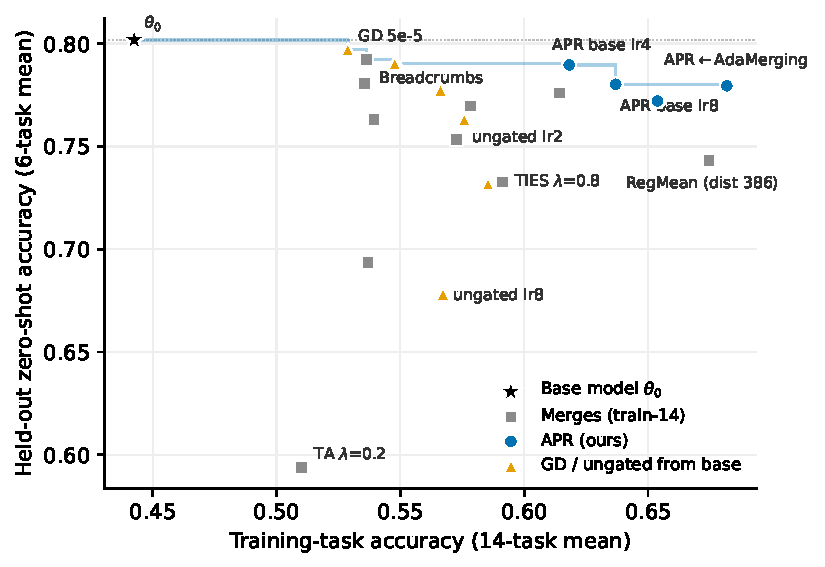
\includegraphics[width=0.40\linewidth]{figs/heldout_frontier.pdf}
\caption{The accuracy--retention trade-off of Table~\ref{tab:clip20heldout}: models built from the $14$ training tasks, evaluated on them ($x$) and zero-shot on the $6$ held-out tasks ($y$; dotted line: the base model). The frontier's high-accuracy half is populated entirely by the anchored refinement; every merge (gray squares) is dominated, and the ungated learning-rate arc (triangles) bends away from it.}
\label{fig:clip20heldout}
\end{figure}

\paragraph{Replay budget, and replication.}
Shrinking the buffer degrades the mean gracefully but the worst task ${\approx}3\times$ faster (Table~\ref{tab:clip20nbudget}, Appendix~\ref{app:clip20}). With just \emph{eight} labels per task, refining the base model reaches $0.632$ ($0.626\pm0.005$ over five draws, above the tuned merge on every draw), and the from-base margin over GD (${\approx}{+}0.05$--$0.06$ mean) is budget-independent---set by the geometry above, not data volume. Five-seed replication of the headline cells (Table~\ref{tab:clip20seeds}, Appendix~\ref{app:clip20}) confirms the single-seed conclusions and sharpens two: the gate's worst-task effect is initialization-dependent (helpful on all five seeds from AdaMerging, $+0.031\pm0.015$; mildly negative from TIES), and the paired margins over plain descent are seed-consistent (e.g.\ $+0.018\pm0.007$ from AdaMerging; $+0.053\pm0.006$ from base at $n=8$).

\paragraph{Summary.}
Five claims survive the twenty-task campaign: (i)~the refinement improves every initialization given---six merges and the base model---with the gain shrinking but never vanishing as the initialization improves; (ii)~the anchored, distance-scaled, clipped step is load-bearing, the gate adding initialization-dependent worst-task repair and held-out retention; (iii)~no anchored run ever fell below its initialization or the floor, while unconstrained descent has catastrophic cells at adjacent rates, overfits small buffers, and can diverge under a buffer redraw; (iv)~eight labels per task beat the tuned merge from the base model alone; (v)~refinement traces an accuracy--retention frontier that merging does not reach (remaining gaps: Appendix~\ref{app:clip20}).

\section{Discussion}
\label{sec:contribution}
This work develops an attribution-patching perspective on replay-guided model merging: the sign of $g_{i,r}v_{i,r}$ answers, coordinate by coordinate, whether moving toward expert $i$ locally reduces the replay loss, and the same condition is a trust-region acceptance rule, so both views motivate one procedure---mask, distance-scale, clip, and apply task-sequentially. Empirically the refinement is a \emph{complement} to merging: it improves every initialization tried, and the strongest results come from composing with the strongest merge. The anchored step retains its advantage and hyperparameter safety at every scale tested; the gate's clearest value appears in fragile regimes---scarce data, fragile tasks, held-out retention. Refining directly from the \emph{pretrained} model reaches merge-level accuracy while staying several times closer to the base weights, a minimal-drift operating point confirmed by a measured accuracy--retention frontier on tasks never merged or refined---in sum, a lightweight bridge between checkpoint-only task arithmetic and full multitask replay fine-tuning.

\subsection*{AI use statement}

% TODO(authors): ICLR 2027 requires this statement; replace the bracketed text
% below with the actual disclosure before submission. It does not count toward
% the page limit.

In this work, we used generative AI tools for [tasks with required disclosure].
We have not used generative AI tools for [other tasks with required disclosure],
and [the rest of the required disclosure tasks] are not applicable to this work.
Additionally, we used generative AI tools for [tasks with recommended
disclosure]. We have reviewed all AI-assisted work. [Elaborate.] We take
responsibility for the final content of this work, including text, claims or
artifacts produced with the aid of generative AI.

\begin{thebibliography}{99}

\bibitem[Davari and Belilovsky(2023)]{davari2023breadcrumbs}
Mohammad Davari and Eugene Belilovsky.
\newblock Model Breadcrumbs: Scaling multi-task model merging with sparse masks.
\newblock \emph{arXiv preprint arXiv:2312.06795}, 2023.

\bibitem[Deep et~al.(2024)]{deep2024della}
Pala Tej Deep, Rishabh Bhardwaj, and Soujanya Poria.
\newblock DELLA-Merging: Reducing interference in model merging through magnitude-based sampling.
\newblock \emph{arXiv preprint arXiv:2406.11617}, 2024.

\bibitem[He et~al.(2024)]{he2024localize}
Shwai He, Runqi Wang, Jindong Wang, Jindong Gu, and Xing Xie.
\newblock Localize-and-Stitch: Efficient model merging via sparse task arithmetic.
\newblock \emph{arXiv preprint arXiv:2408.13656}, 2024.

\bibitem[He et~al.(2025)]{he2025mergebench}
Yifei He, Siqi Zeng, Yuzheng Hu, Rui Yang, Tong Zhang, and Han Zhao.
\newblock MergeBench: A benchmark for merging domain-specialized LLMs.
\newblock In \emph{Advances in Neural Information Processing Systems (Datasets and Benchmarks Track)}, 2025.

\bibitem[Ilharco et~al.(2022)]{ilharco2022taskarithmetic}
Gabriel Ilharco, Marco Tulio Ribeiro, Mitchell Wortsman, Suchin Gururangan, Ludwig Schmidt, Hannaneh Hajishirzi, and Ali Farhadi.
\newblock Editing models with task arithmetic.
\newblock \emph{arXiv preprint arXiv:2212.04089}, 2022.

\bibitem[Jin et~al.(2023)]{jin2023regmean}
Xisen Jin, Xiang Ren, Daniel Preotiuc-Pietro, and Pengxiang Cheng.
\newblock Dataless knowledge fusion by merging weights of language models.
\newblock In \emph{International Conference on Learning Representations}, 2023.

\bibitem[Kong et~al.(2024)]{kong2024apl}
Fanshuang Kong, Richong Zhang, and Ziqiao Wang.
\newblock Activated parameter locating via causal intervention for model merging.
\newblock \emph{arXiv preprint arXiv:2408.09485}, 2024.

\bibitem[Kramar et~al.(2024)]{kramar2024atpstar}
Janos Kramar, Tom Lieberum, Rohin Shah, and Neel Nanda.
\newblock AtP*: An efficient and scalable method for localizing language model behavior to components.
\newblock \emph{arXiv preprint arXiv:2403.00745}, 2024.

\bibitem[Liu et~al.(2019)]{liu2019roberta}
Yinhan Liu, Myle Ott, Naman Goyal, Jingfei Du, Mandar Joshi, Danqi Chen, Omer Levy, Mike Lewis, Luke Zettlemoyer, and Veselin Stoyanov.
\newblock RoBERTa: A robustly optimized BERT pretraining approach.
\newblock \emph{arXiv preprint arXiv:1907.11692}, 2019.

\bibitem[Lu et~al.(2024)]{lu2024twin}
Zhenyi Lu, Chengxu Yin, Wujie Wang, and Xuebo Liu.
\newblock Twin-Merging: Dynamic integration of modular expertise in model merging.
\newblock \emph{arXiv preprint arXiv:2406.15479}, 2024.

\bibitem[Matena and Raffel(2022)]{matena2022fisher}
Michael S. Matena and Colin A. Raffel.
\newblock Merging models with Fisher-weighted averaging.
\newblock In \emph{Advances in Neural Information Processing Systems}, 2022.

\bibitem[Radford et~al.(2021)]{radford2021clip}
Alec Radford, Jong Wook Kim, Chris Hallacy, Aditya Ramesh, Gabriel Goh, Sandhini Agarwal, Girish Sastry, Amanda Askell, Pamela Mishkin, Jack Clark, Gretchen Krueger, and Ilya Sutskever.
\newblock Learning transferable visual models from natural language supervision.
\newblock In \emph{International Conference on Machine Learning}, 2021.

\bibitem[Raffel et~al.(2020)]{raffel2020t5}
Colin Raffel, Noam Shazeer, Adam Roberts, Katherine Lee, Sharan Narang, Michael Matena, Yanqi Zhou, Wei Li, and Peter J. Liu.
\newblock Exploring the limits of transfer learning with a unified text-to-text transformer.
\newblock \emph{Journal of Machine Learning Research}, 21(140):1--67, 2020.

\bibitem[Sanh et~al.(2019)]{sanh2019distilbert}
Victor Sanh, Lysandre Debut, Julien Chaumond, and Thomas Wolf.
\newblock DistilBERT, a distilled version of BERT: smaller, faster, cheaper and lighter.
\newblock \emph{arXiv preprint arXiv:1910.01108}, 2019.

\bibitem[Sundararajan et~al.(2017)]{sundararajan2017ig}
Mukund Sundararajan, Ankur Taly, and Qiqi Yan.
\newblock Axiomatic attribution for deep networks.
\newblock In \emph{International Conference on Machine Learning}, 2017.

\bibitem[Syed et~al.(2024)]{syed2024attributionpatching}
Aaquib Syed, Can Rager, and Arthur Conmy.
\newblock Attribution patching outperforms automated circuit discovery.
\newblock \emph{arXiv preprint arXiv:2310.10348}, 2024.

\bibitem[Tang et~al.(2024)]{tang2024fusionbench}
Anke Tang, Li Shen, Yong Luo, Liang Ding, Han Hu, Bo Du, and Dacheng Tao.
\newblock FusionBench: A comprehensive benchmark of deep model fusion.
\newblock \emph{arXiv preprint arXiv:2406.03280}, 2024.

\bibitem[Wang et~al.(2018)]{wang2018glue}
Alex Wang, Amanpreet Singh, Julian Michael, Felix Hill, Omer Levy, and Samuel R. Bowman.
\newblock GLUE: A multi-task benchmark and analysis platform for natural language understanding.
\newblock In \emph{Proceedings of the 2018 EMNLP Workshop BlackboxNLP}, 2018.

\bibitem[Wang et~al.(2019)]{wang2019superglue}
Alex Wang, Yada Pruksachatkun, Nikita Nangia, Amanpreet Singh, Julian Michael, Felix Hill, Omer Levy, and Samuel R. Bowman.
\newblock SuperGLUE: A stickier benchmark for general-purpose language understanding systems.
\newblock In \emph{Advances in Neural Information Processing Systems}, 2019.

\bibitem[Wang et~al.(2024)]{wang2024tall}
Ke Wang, Nikolaos Dimitriadis, Guillermo Ortiz-Jim\'enez, Fran\c{c}ois Fleuret, and Pascal Frossard.
\newblock Localizing task information for improved model merging and compression.
\newblock In \emph{International Conference on Machine Learning}, 2024.

\bibitem[Wortsman et~al.(2022)]{wortsman2022modelsoups}
Mitchell Wortsman, Gabriel Ilharco, Samir Yitzhak Gadre, Rebecca Roelofs, Raphael Gontijo-Lopes, Ari S. Morcos, Hongseok Namkoong, Ali Farhadi, Yair Carmon, Simon Kornblith, and Ludwig Schmidt.
\newblock Model soups: Averaging weights of multiple fine-tuned models improves accuracy without increasing inference time.
\newblock In \emph{International Conference on Machine Learning}, 2022.

\bibitem[Xiao et~al.(2024)]{xiao2024lmcocktail}
Shitao Xiao, Zheng Liu, Peitian Zhang, and Xingrun Xing.
\newblock LM-Cocktail: Resilient tuning of language models via model merging.
\newblock In \emph{Findings of the Association for Computational Linguistics: ACL 2024}, 2024.

\bibitem[Yadav et~al.(2023)]{yadav2023ties}
Prateek Yadav, Derek Tam, Leshem Choshen, Colin Raffel, and Mohit Bansal.
\newblock TIES-Merging: Resolving interference when merging models.
\newblock \emph{arXiv preprint arXiv:2306.01708}, 2023.

\bibitem[Yang et~al.(2024)]{yang2024adamerging}
Enneng Yang, Zhenyi Wang, Li Shen, Shiwei Liu, Guibing Guo, Xingwei Wang, and Dacheng Tao.
\newblock AdaMerging: Adaptive model merging for multi-task learning.
\newblock \emph{arXiv preprint arXiv:2310.02575}, 2024.

\bibitem[Yu et~al.(2023)]{yu2023dare}
Le Yu, Bowen Yu, Haiyang Yu, Fei Huang, and Yongbin Li.
\newblock Language models are Super Mario: Absorbing abilities from homologous models as a free lunch.
\newblock \emph{arXiv preprint arXiv:2311.03099}, 2023.

\bibitem[Zeng et~al.(2025)]{zeng2025taskvectorbases}
Zihan Zeng, Jiahui Chen, Lei Li, and Min Zhang.
\newblock Efficient model editing with task vector bases: A theoretical framework and scalable approach.
\newblock \emph{arXiv preprint arXiv:2502.01015}, 2025.

\end{thebibliography}


\appendix

\section{Box-Distance Monotonicity and the Expert Box}
\label{app:box-theory}

This appendix proves the general geometric result behind
Corollary~\ref{cor:algorithm-box-distance}. The statement is
self-contained: $x_1,\dots,x_n$ are arbitrary points in $\mathbb{R}^D$
(in the application, the task experts $\theta_1,\dots,\theta_T$), and the
superscript $d$ indexes coordinates.

\begin{theorem}[Box-distance monotonicity under coordinatewise movement toward a hull point]
\label{thm:box-distance-monotonicity}
Let \(x_1,\dots,x_n\in \mathbb{R}^D\). Define the axis-aligned box hull
\[
B:=\prod_{d=1}^D [m_d,M_d],
\qquad
m_d:=\min_{1\le j\le n} x_j^d,
\qquad
M_d:=\max_{1\le j\le n} x_j^d.
\]
Let \(y,z\in \mathbb{R}^D\). Suppose that there exists some
\(i\in\{1,\dots,n\}\) such that, for every coordinate \(d\in\{1,\dots,D\}\),
the point \(z^d\) lies between \(x_i^d\) and \(y^d\). Equivalently,
\[
|z^d-x_i^d|\le |y^d-x_i^d|
\]
and \(z^d-x_i^d\) has the same sign as \(y^d-x_i^d\), allowing equality.

Then, for every \(1\le p\le \infty\),
\[
d_p(z,B)\le d_p(y,B),
\]
where \(d_p(u,B)\) denotes the distance from \(u\) to \(B\) with respect to
the \(\ell^p\)-norm.
\end{theorem}

\begin{proof}
For each coordinate \(d\), set
\[
I_d:=[m_d,M_d].
\]
Since \(x_i\in B\), we have
\[
x_i^d\in I_d
\]
for every \(d\).

Define the one-dimensional distance function
\[
\delta_d(t):=\operatorname{dist}(t,I_d)
=
\inf_{s\in I_d}|t-s|.
\]

We first prove the following elementary one-dimensional claim.

\medskip

\noindent
\textbf{Claim.}
Let \(I=[m,M]\subset \mathbb{R}\), let \(c\in I\), and suppose that
\(z\) lies between \(c\) and \(y\). Then
\[
\operatorname{dist}(z,I)\le \operatorname{dist}(y,I).
\]

\medskip

\noindent
Indeed, if \(y\in I\), then since \(c\in I\) and \(I\) is an interval,
every point between \(c\) and \(y\) also lies in \(I\). Hence \(z\in I\), so
\[
\operatorname{dist}(z,I)=0=\operatorname{dist}(y,I).
\]

If \(y>M\), then
\[
\operatorname{dist}(y,I)=y-M.
\]
Since \(z\) lies between \(c\in I\) and \(y>M\), we have \(z\le y\). If
\(z\le M\), then \(\operatorname{dist}(z,I)=0\). If \(z>M\), then
\[
\operatorname{dist}(z,I)=z-M\le y-M=\operatorname{dist}(y,I).
\]
The case \(y<m\) is symmetric. This proves the claim.

\medskip

Now apply the claim coordinatewise with
\[
I=I_d,
\qquad
c=x_i^d.
\]
Because \(z^d\) lies between \(x_i^d\) and \(y^d\), we obtain
\[
\delta_d(z^d)\le \delta_d(y^d)
\]
for every \(d\in\{1,\dots,D\}\).

Next, distance to an axis-aligned box separates coordinatewise. Namely, for
\(1\le p<\infty\),
\[
d_p(u,B)
=
\left(
\sum_{d=1}^D \delta_d(u^d)^p
\right)^{1/p},
\]
and for \(p=\infty\),
\[
d_\infty(u,B)
=
\max_{1\le d\le D}\delta_d(u^d).
\]
This follows because the closest point of \(B\) to \(u\) is obtained by
clipping each coordinate \(u^d\) to the interval \(I_d=[m_d,M_d]\).

Since
\[
\delta_d(z^d)\le \delta_d(y^d)
\]
for every \(d\), monotonicity of the \(\ell^p\)-norm on the nonnegative
orthant gives
\[
d_p(z,B)\le d_p(y,B).
\]
This proves the theorem.
\end{proof}

The box hull \(B\) may look like a loose relaxation of the ordinary convex
hull of the experts, but it is canonical in its own right: it is the
smallest set containing the experts that is convex with respect to
\(\ell^1\)-geodesics.

\begin{proposition}
\label{prop:l1-geodesic-box-hull}
The set \(B\) is the \(\ell^1\)-geodesic convex hull of
\(\{x_1,\dots,x_n\}\).
\end{proposition}

\begin{proof}
For \(a,b\in \mathbb{R}^D\), define the \(\ell^1\)-metric interval between
\(a\) and \(b\) by
\[
I_1(a,b)
:=
\{u\in\mathbb{R}^D:
\|a-u\|_1+\|u-b\|_1=\|a-b\|_1\}.
\]
We claim that
\[
I_1(a,b)
=
\prod_{d=1}^D
[\min(a^d,b^d),\max(a^d,b^d)].
\]

Indeed, by the triangle inequality in one dimension,
\[
|a^d-u^d|+|u^d-b^d|\ge |a^d-b^d|
\]
for each coordinate \(d\). Summing over \(d\), equality in the
\(\ell^1\)-triangle inequality holds if and only if equality holds in every
coordinate. In one dimension, equality holds precisely when \(u^d\) lies
between \(a^d\) and \(b^d\). Hence the displayed formula for \(I_1(a,b)\)
follows.

Now \(B\) is clearly \(\ell^1\)-geodesically convex: if \(a,b\in B\), then
every point coordinatewise between \(a\) and \(b\) also lies in \(B\).

It remains to show minimality. Let \(C\subseteq \mathbb{R}^D\) be any
\(\ell^1\)-geodesically convex set containing \(x_1,\dots,x_n\). Since
\(C\) is closed under \(\ell^1\)-metric intervals, it is closed under taking
coordinatewise boxes between pairs of its points. In particular, if
\(a,b\in C\), then both the coordinatewise minimum
\[
a\wedge b
:=
(\min(a^1,b^1),\dots,\min(a^D,b^D))
\]
and the coordinatewise maximum
\[
a\vee b
:=
(\max(a^1,b^1),\dots,\max(a^D,b^D))
\]
belong to \(C\).

By induction, \(C\) therefore contains the coordinatewise minimum
\[
m:=(m_1,\dots,m_D)
\]
and the coordinatewise maximum
\[
M:=(M_1,\dots,M_D)
\]
of the points \(x_1,\dots,x_n\). Since \(C\) is \(\ell^1\)-geodesically
convex, it contains the entire \(\ell^1\)-metric interval between \(m\) and
\(M\). But
\[
I_1(m,M)
=
\prod_{d=1}^D [m_d,M_d]
=
B.
\]
Therefore every \(\ell^1\)-geodesically convex set containing
\(x_1,\dots,x_n\) also contains \(B\). Hence \(B\) is the smallest such set,
i.e.
\[
B=\operatorname{gconv}_{\ell^1}\{x_1,\dots,x_n\}.
\]
\end{proof}


We can now state and prove the guarantee for Algorithm~\ref{alg:expert-gated-refinement} used in Section~\ref{sec:replay-refinement}.

\begin{corollary}[Box-distance monotonicity of the sequential refinement]
\label{cor:algorithm-box-distance}
Let
\[
B_{\mathrm{exp}}
:=
\prod_{r=1}^d
[\underline{\theta}_r,\overline{\theta}_r],
\qquad
\underline{\theta}_r := \min_{j\in\tasks}\theta_{j,r},
\qquad
\overline{\theta}_r := \max_{j\in\tasks}\theta_{j,r},
\]
be the axis-aligned box hull of the task experts. Then every
within-sweep update of Algorithm~\ref{alg:expert-gated-refinement} is
non-expansive in distance to the expert box: for every $1\le p\le\infty$,
\[
    d_p\!\left(\theta^{(s,k)},B_{\mathrm{exp}}\right)
    \le
    d_p\!\left(\theta^{(s,k-1)},B_{\mathrm{exp}}\right).
\]
Consequently, after any number $S$ of sweeps,
\[
    d_p\!\left(\theta^{(S)},B_{\mathrm{exp}}\right)
    \le
    d_p\!\left(\theta^{(0)},B_{\mathrm{exp}}\right)
    \qquad\text{for every }1\le p\le\infty.
\]
\end{corollary}

\begin{proof}
Fix a sweep $s$, a within-sweep index $k$, and let $i=\pi_s(k)$. We first
verify the hypothesis of Theorem~\ref{thm:box-distance-monotonicity} with
\[
    y=\theta^{(s,k-1)},
    \qquad
    z=\theta^{(s,k)},
    \qquad
    x_i=\theta_i.
\]
It is enough to check that, for every coordinate $r$, the new coordinate
$\theta_r^{(s,k)}$ lies between the previous coordinate
$\theta_r^{(s,k-1)}$ and the expert coordinate $\theta_{i,r}$.

Write $v_r=v_{i,r}^{(s,k)}=\theta_{i,r}-\theta_r^{(s,k-1)}$. If the gate is
off, then $m_{i,r}^{(s,k)}=0$, hence $u_{i,r}^{(s,k)}=0$, and the coordinate
is unchanged. If the gate is on, then
\[
    g_{i,r}^{(s,k)} v_r < -\epsilon_{\mathrm{gate}} \le 0,
\]
so $-g_{i,r}^{(s,k)}$ has the same sign as $v_r$. Therefore the raw update
$\widetilde u_{i,r}^{(s,k)}=-g_{i,r}^{(s,k)}|v_r|m_{i,r}^{(s,k)}$ points in
the same direction as $v_r$. Multiplication by $\eta\ge0$ preserves this
direction, possibly making the update zero, and the symmetric clip in
Equation~\eqref{eq:clipped-update} gives an applied update with the same weak sign as $v_r$ and magnitude at most $|v_r|$.
Thus there is an $\alpha_{i,r}^{(s,k)}\in[0,1]$ such that
\[
    u_{i,r}^{(s,k)}=\alpha_{i,r}^{(s,k)}v_{i,r}^{(s,k)}.
\]
The same representation is assumed directly in the optional post-processing
case. Hence
\[
    \theta_r^{(s,k)}
    =
    \theta_r^{(s,k-1)}
    +
    \alpha_{i,r}^{(s,k)}
    \bigl(\theta_{i,r}-\theta_r^{(s,k-1)}\bigr),
\]
so $\theta_r^{(s,k)}$ lies between $\theta_r^{(s,k-1)}$ and $\theta_{i,r}$.

The box $B_{\mathrm{exp}}$ is exactly the axis-aligned hull of the expert
points $\theta_1,\dots,\theta_T$. Therefore
Theorem~\ref{thm:box-distance-monotonicity} gives
\[
    d_p\!\left(\theta^{(s,k)},B_{\mathrm{exp}}\right)
    \le
    d_p\!\left(\theta^{(s,k-1)},B_{\mathrm{exp}}\right)
\]
for every $1\le p\le\infty$. Chaining this inequality over
$k=1,\dots,T$ and over sweeps $s=0,\dots,S-1$ gives the final statement.
\end{proof}


\section{Method Details: Sequential Scheduling}
\label{app:method}
This appendix reproduces the extended discussion of the update rule and its sequential scheduling, compressed in Section~\ref{sec:replay-refinement}.

This baseline treats the merge like any other initialization and lets the replay gradients move each coordinate freely, with nothing tying the refined model to the known task experts. The central departure of our method is precisely this anchoring: rather than taking a free gradient step, every coordinate of the update is tied to the corresponding task expert. For each task $i$ and coordinate $r$ we (i) weight the negative-gradient step by the current distance $|v_{i,r}|$ to the expert, so that coordinates already close to the expert barely move while coordinates far from it move more; (ii) keep the step only where it moves the model \emph{toward} the expert, discarding coordinates whose replay gradient would pull away from it; and (iii) clip the resulting step to the expert-distance trust region so that a single update can never overshoot the expert. These three operations---expert-distance weighting, the expert-agreement gate, and the trust-region clip---are what distinguish the refinement from ordinary replay gradient descent, and together they keep the whole refinement anchored to the known experts rather than letting it drift.

A secondary and comparatively minor design choice concerns how the per-task updates are scheduled within a refinement step. An aggregated expert-guided update would compute all $u_i$ at $\theta^{(s)}$ and then apply $\eta\sum_i u_i$ at once; we instead apply each task's update immediately after computing it, so that its gradient, expert direction, and gate are evaluated at the same model state to which it is applied.

The robustness of the refinement comes primarily from the expert anchoring rather than from this scheduling: the distance weighting and gate keep every coordinate pointed at its expert, and the trust-region clip caps how far it can travel. The immediate application of each update, though secondary to the anchoring, has two motivations of its own. First, each update is applied at the same local model state on which its gradient, expert direction, and gate were computed. Second, the trust-region clipping in Equation~\eqref{eq:clipped-update} controls each single-task movement before the next task sees the modified model, rather than allowing several task vectors to accumulate into one larger coordinate step. Because the clip is applied \emph{after} the learning-rate scaling, the per-coordinate movement is bounded by $|v_{i,r}^{(s,k)}|$ for any $\eta$; for $\le 1$ a single update can never overshoot the expert in a coordinate, so the refinement stays within the expert-distance trust region and cannot diverge no matter how large $\eta$ is. The learning rate then controls only how many coordinates are driven to the trust-region boundary, not the maximum per-coordinate step size. The sequential rule still does not guarantee Pareto improvement across tasks, because an update that helps task $i$ can hurt task $j$. We therefore treat task ordering, cross-task interference, and worst-task retention as explicit diagnostics rather than as consequences of the gate alone. In practice, one can also normalize $u_i^{(s,k)}$ by tensor-wise RMS before applying the single-task update; the defining operation remains the coordinate gate in Equation~\eqref{eq:ap-gate}, whether it is read as an attribution-patching sign or as a trust-region acceptance rule. Under either reading the procedure is the single algorithm summarized in Algorithm~\ref{alg:expert-gated-refinement}.


\section{Extended Experimental Protocol}
\label{app:protocol}
This appendix expands the protocol of Section~\ref{sec:protocol}: benchmark positioning, development order, secondary tracks, replay sampling, the full baseline roster, planned task-similarity diagnostics, the ablation grid, and the full hypothesis statements.

\paragraph{Benchmark settings.}
The multi-head GLUE-8 benchmark (CoLA, SST-2, MRPC, STS-B, QQP, MNLI, QNLI, RTE, excluding WNLI as is common) \citep{wang2018glue} uses RoBERTa-base as the encoder backbone \citep{liu2019roberta}: the shared encoder is merged and evaluated with each task's own trained head. This multi-head setup is convenient and common, but it assumes oracle task identity at evaluation time and should not be the only evidence for the method. The recent merging literature evaluates on three benchmark families---CLIP/ViT vision task-vector suites, GLUE and text-to-text NLP, and decoder-only LLM merging, the last standardized by MergeBench with released full-parameter Llama/Gemma experts \citep{radford2021clip,ilharco2022taskarithmetic,tang2024fusionbench,wang2019superglue,raffel2020t5,yu2023dare,he2025mergebench}---and we position the proposal against all three (protocol details in Section~\ref{sec:protocol}).

\paragraph{Proof-of-concept order.}
Development proceeds from small to large: a distilled-encoder smoke test on MRPC/STS-B \citep{sanh2019distilbert}, a RoBERTa-base three-task study (MRPC/STS-B/SST-2: one related sentence-pair pair plus a less-related single-sentence control), and the full GLUE-8 scale-up with all feasible baselines, where CoLA and RTE require multiple seeds and MNLI dominates the compute budget. A systematic pairwise and subset study (all pairwise merges, related/stress subsets, the entailment cluster) remains planned as a guard against favorable task selection; distilled models are used only for debugging, never as evidence.

\paragraph{Secondary benchmark settings.}
Three secondary tracks address the limitations of multi-head GLUE. A shared-output NLP track evaluates GLUE in text-to-text format with T5-style models, so the merged model uses a common generation head rather than task-specific classifiers \citep{wang2019superglue,raffel2020t5} (results in Section~\ref{sec:t5}). A CLIP/ViT vision track evaluates the standard task-vector image-classification suite---SUN397, Cars, RESISC45, EuroSAT, SVHN, GTSRB, MNIST, DTD---testing a different modality, different loss geometry, and stronger domain shifts \citep{radford2021clip,ilharco2022taskarithmetic,tang2024fusionbench}, together with its twenty-task extension \citep{wang2024tall} (adding CIFAR-10/100, STL10, Flowers102, Oxford Pets, PCAM, FER2013, EMNIST, Food101, FashionMNIST, KMNIST, RenderedSST2), which probes the high-interference regime in which merging degrades most (results in Section~\ref{sec:clip20}). A decoder-only LLM track adopts the MergeBench setting \citep{he2025mergebench}: published full-parameter domain experts for the Llama and Gemma families share a common pretrained checkpoint, so task vectors and merge-to-expert directions are well defined and no expert training is required on our side. We begin at a full-fine-tuning-feasible scale (Llama-3.2-3B) with the strongly interfering instruction/mathematics/coding triple---the worst-task-retention stress regime in which the gate helped most on CLIP/ViT---using judge-free automatic metrics (verifiable instruction constraints, exact match on grade-school mathematics, functional-correctness pass rates on code) and subsampled evaluation sets during hyperparameter search, since generation-based evaluation is the dominant cost.

\paragraph{Replay data.}
For refinement, we use $n \in \{4,8,16,32,64,128\}$ replay examples per task. Replay examples are sampled from training data or from a held-out split separated from the final validation split. For classification tasks, replay buffers should be class-balanced whenever possible; for imbalanced tasks such as QQP and for small tasks such as RTE, we report the exact sampling procedure. We report sensitivity to the number of replay examples, variation across replay samples, and the area under the replay-budget curve rather than only the best tuned replay size.

\paragraph{Baselines.}
Because the proposed method uses labeled replay buffers, baselines are grouped by data regime: \emph{checkpoint-only} (pretrained encoder, single-task experts, uniform averaging, task arithmetic, Fisher merging, TIES, DARE, DELLA-style sampling, Model Breadcrumbs, Localize-and-Stitch); \emph{data-dependent but label-free} (RegMean, AdaMerging, APL); \emph{labeled-replay} (ordinary replay gradient descent from the same initialization, distance-scaled descent without the gate, head-only calibration, encoder and encoder-plus-head replay fine-tuning, multitask replay fine-tuning from the pretrained checkpoint and from the merge); and \emph{sanity controls} (inverted gate, density-matched random gate, wrong-expert directions, shuffled labels, frozen first-step gates, and the aggregated-$U$ variant). All labeled-replay baselines use the same replay examples, the same number of gradient evaluations where possible, and the same hyperparameter search budget---essential because the strongest alternative explanation for a positive result is simply that the method performs supervised post-merge replay fine-tuning.

\paragraph{Task-similarity and interference analysis.}
We group GLUE-8 into interpretable clusters---paraphrase/similarity $\{\mathrm{MRPC},\mathrm{QQP},\mathrm{STS\mbox{-}B}\}$, entailment $\{\mathrm{MNLI},\mathrm{QNLI},\mathrm{RTE}\}$, single-sentence $\{\mathrm{CoLA},\mathrm{SST\mbox{-}2}\}$---and test whether the gated refinement helps most in related clusters, where movement toward one expert is more likely to be compatible with the others. Planned diagnostics include task-vector cosine similarity, attribution-sign agreement, and the cross-task interference matrix $C_{j\leftarrow i}^{(s,k)}=\langle\nabla_\theta \loss_j(\theta^{(s,k-1)};\data_j^{\mathrm{probe}}),\,u_i^{(s,k)}\rangle$, whose sign indicates whether task $i$'s update is locally predicted to help or hurt task $j$.

\subsection{Ablations and Diagnostics}
The planned ablations cover: \textbf{gate sign and necessity} (proposed gate vs.\ no gate, inverted gate, and a density-matched random mask); \textbf{gate confidence and granularity} ($\epsilon_{\mathrm{gate}}$, coordinate vs.\ tensor or block gates, top-$k$ attribution masks, sign-stability masks); \textbf{the sequential rule} (immediate vs.\ aggregated-$U$; fixed, cyclic, and random task order); \textbf{distance scaling} (ordinary replay GD, ungated distance-scaled descent, direct interpolation $u_i\propto m_i v_i$, full gated update); \textbf{clipping and normalization} (none, tensor-wise RMS, global-norm clipping, validation line search); \textbf{replay budget and variance}; \textbf{refinement horizon} $S\in\{0,1,2,5,10\}$; \textbf{expansion point} (fresh gates every update vs.\ frozen first-sweep gates); and \textbf{label/expert sanity checks} (shuffled replay labels, wrong-expert directions).

\subsection{Hypotheses}
The project evaluates five hypotheses:
\begin{description}[style=nextline,leftmargin=1.5em,labelindent=0pt]
    \item[H1: Attribution-patching signs predict useful expert directions.] Coordinates with $g_{i,r}v_{i,r}<0$ should be more likely to reduce task $i$'s loss when moved toward expert $i$ than those with $g_{i,r}v_{i,r}>0$.
    \item[H2: Expert-guided replay refinement improves task arithmetic.] From the same initialization and replay budget, the gated update should outperform ordinary and ungated distance-scaled replay gradient descent.
    \item[H3: Sequential single-task updates improve worst-task retention.] Immediate application should reduce overshoot and stale-gradient effects relative to aggregated-$U$.
    \item[H4: Benefits are larger for related tasks.] Gains should concentrate in related clusters, especially MRPC/QQP/STS-B.
    \item[H5: Gains are not GLUE-specific.] A positive GLUE result should transfer at least partially to a shared-head text-to-text setting, to CLIP/ViT, or to MergeBench decoder merging.
\end{description}


\section{Multi-Head GLUE: Extended Results}
\label{app:glue}
This appendix reproduces the full discussion of the multi-head RoBERTa experiments summarized at the start of Section~\ref{sec:results}.

We report initial experiments in the RoBERTa-base multi-head setting (oracle task identity at evaluation). Unless noted, refinement uses $S$ sweeps from the task-arithmetic merge with the corrected trust region applied \emph{after} the learning rate (Eq.~\eqref{eq:clipped-update}) and threshold $\epsilon_{\mathrm{gate}}=0$. Each method family (ordinary replay gradient descent, the proposed gated update, and the ungated distance-scaled update) is given its own learning-rate search of equal size; we report the best configuration per family by mean normalized retention (Eq.~\eqref{eq:normalized-retention}). Section~\ref{sec:mergebaselines} additionally compares the refinement against interference-aware and label-free merge baselines, and composes it with them. Section~\ref{sec:t5} then removes the multi-head assumption entirely, repeating the core comparisons on a text-to-text T5 track in which every task decodes through a single shared generation head.

These results carry three qualifications. First, the hyperparameter-sweep cells are single-seed, with a run-to-run spread of roughly $\pm0.02$ mean retention (Table~\ref{tab:glue8}), so sweep-level differences smaller than that should not be read as orderings; the headline configurations are replicated over five replay-buffer seeds (Table~\ref{tab:multiseed}). Second, hyperparameters (learning rate, and in Section~\ref{sec:mergebaselines} also $\lambda$, sparsity, and density) are selected \emph{per family} by mean normalized retention on the evaluation split---a uniform and therefore fair rule, but oracle selection; the stricter protocol, in which every labeled method selects its hyperparameters on the replay buffer alone, is applied in Table~\ref{tab:matched}. Third, the multi-head GLUE setting assumes oracle task identity.

\paragraph{Three-task proof of concept.}
On the MRPC/STS-B/SST-2 triple ($n=64$ replay examples per task, $S=5$), all refinement families recover most of the gap from the task-arithmetic merge ($0.558$) toward the experts and are statistically tied at their tuned optima (Table~\ref{tab:poc3}). The decisive difference is learning-rate robustness: the gated update peaks at a much larger step ($\eta=64$) and remains stable there, whereas the ungated update---identical except for the gate---\emph{diverges} at the same learning rate ($-1.07$). The gate acts as a protective mask that makes large steps safe by suppressing locally loss-increasing expert directions.

\begin{table}[t]
\centering
\caption{Three-task RoBERTa-base proof of concept (MRPC, STS-B, SST-2; $n=64$, $S=5$). Mean normalized retention; best learning rate per family. Left: best configuration, mean $\pm$ std over five seeds. Right: a single-seed contrast at a large fixed learning rate, isolating the gate's effect.}
\label{tab:poc3}
\begin{tabular}{lcc}
\toprule
Method & Best mean NormRet ($\pm$ std) & at $\eta=64$ (1 seed) \\
\midrule
Task-arithmetic merge & $0.558$ & --- \\
Ordinary replay GD & $0.831\pm0.005$ & --- \\
Ungated distance-scaled (no gate) & $0.835\pm0.017$ & $-1.07$ (diverges) \\
\textbf{APR (gated, proposed)} & $\mathbf{0.840\pm0.021}$ & $\mathbf{0.849}$ (stable) \\
\bottomrule
\end{tabular}
\end{table}

\paragraph{GLUE-8 scale-up.}
Merging all eight experts (one consistent RoBERTa-base fine-tuning source) is far more interference-prone: the task-arithmetic merge attains only $0.320$, with MRPC driven below the pretrained baseline. Expert anchoring matters more here: both anchored updates clearly outperform ordinary replay gradient descent, especially on worst-task retention (Table~\ref{tab:glue8}). The gate is approximately performance-neutral relative to the ungated update on mean retention---the ordering flips between the two budgets and the gaps are within single-seed noise---but it again widens the safe learning-rate range (stable through $\eta=16$, versus an ungated peak at $\eta=2\text{--}4$ and divergence by $\eta\gtrsim 8\text{--}16$). MRPC and CoLA remain the persistent worst tasks; QQP, STS-B, MNLI, and QNLI recover to $0.78\text{--}0.86$.

A caveat on the boundary of that safe range. At $\eta=32$ the gated update attained $0.614$ (worst $0.142$) in one run, but an identically configured re-run collapsed to $-0.093$ (worst $-3.467$, MRPC); we therefore report the stable $\eta=16$ configuration. The replay gradients are deterministic (computed in \texttt{eval} mode, so no dropout noise enters), which localises the cause to floating-point non-associativity on the GPU: atomics in the embedding backward pass and state-dependent kernel selection perturb the gradient in its last bits, the gate \emph{discretises} the perturbation (coordinates with $g_{i,r}v_{i,r}\approx 0$ flip sign), and near the divergence boundary the trajectories separate. The trust region guarantees that large steps remain \emph{bounded} (Section~\ref{sec:replay-refinement}), but near the critical learning rate it does not make the outcome \emph{reproducible}; reported learning rates should be interior to the stable range, not at its edge.

\begin{table}[t]
\centering
\caption{GLUE-8 (all eight tasks, RoBERTa-base, single seed). Best mean normalized retention per family (worst-task retention in parentheses); the task-arithmetic merge baseline is $0.320$ (worst $-0.175$). APR is reported at its largest stable learning rate, $\eta=16$; the $\eta=32$ configuration reached $0.614$ once but is not reproducible (see text).}
\label{tab:glue8}
\begin{tabular}{lcc}
\toprule
Method & $n{=}64,\,S{=}5$ & $n{=}32,\,S{=}10$ \\
\midrule
Ordinary replay GD & $0.574\ (0.04)$ & $0.588\ (0.04)$ \\
Ungated distance-scaled (no gate) & $\mathbf{0.637}\ (0.15)$ & $0.607\ (0.05)$ \\
\textbf{APR (gated, proposed)} & $0.595\ (0.11)$ & $\mathbf{0.617}\ (0.05)$ \\
\bottomrule
\end{tabular}
\end{table}

\paragraph{What the attribution gate is and is not doing.}
Two diagnostics temper the interpretation of the gate. First, it keeps a strikingly stable $\approx 36\%$ of coordinates across sweeps, tasks, and learning rates, and a control attributes most of this to gradient sparsity rather than expert geometry: roughly $31\%$ of encoder coordinates are word-embedding rows for tokens absent from the replay buffer (exactly zero gradient, always masked), and a random direction of matched magnitudes reproduces almost the same density ($0.345$ vs.\ $0.361$ for the true expert direction). Second, the trust-region clip is almost never active at useful learning rates ($<0.1\%$ of gated coordinates)---a rare-event safeguard, not a routine operation. On GLUE the gate's measurable benefit is therefore learning-rate robustness rather than a higher peak score.

A density-matched random mask makes this concrete. Over five replay-buffer seeds on GLUE-8 (Table~\ref{tab:multiseed}), the true gate ($0.542\pm0.062$) is statistically indistinguishable from---indeed nominally worse than---a random gate of the same density ($0.568\pm0.031$), and both trail the ungated update ($0.593\pm0.040$): on this modality the gate's \emph{sign} carries no signal beyond its density, as the embedding-sparsity account predicts. The same control behaves oppositely on CLIP (Section~\ref{sec:mergebaselines}), sharpening the modality split: the attribution sign is informative where gradients are dense, and vacuous where the replay buffer leaves most coordinates without gradient.


\section{CLIP-8: Extended Results}
\label{app:clip8}
This appendix reproduces the full discussion of the eight-task CLIP/ViT experiments, including per-task scores and the replay-budget and horizon studies.

\paragraph{CLIP/ViT vision track.}
We next test transfer to the standard eight-task CLIP task-vector suite (SUN397, Cars, RESISC45, EuroSAT, SVHN, GTSRB, MNIST, DTD) with a ViT-B/32 backbone: the image encoder is merged while each task keeps a \emph{frozen} zero-shot head derived from the CLIP text encoder; the experts are publicly available fine-tuned encoders, merged with uniform $\lambda_i=0.3$ (later shown over-scaled; Section~\ref{sec:mergebaselines}). Refinement uses $n=64$, $S=5$, $\gamma=1$ (single seed). This is a stronger test than GLUE---a different modality, dense gradients without the word-embedding sparsity above, larger domain shifts---and the merge is weak here ($0.270$ mean, $-0.527$ worst; SUN397 and Cars fall \emph{below} the zero-shot backbone). All three families recover substantial ground, but---in contrast to GLUE-8---the gate attains the best mean retention and, \emph{among the three replay-refinement families}, the only positive worst-task retention (Table~\ref{tab:clip8}); the latter does not extend to merge methods generally, since tuned task arithmetic, Breadcrumbs, and TIES all achieve it with no data (Section~\ref{sec:mergebaselines}). The gated update lifts the merge from $0.270$ to $0.598$ mean and from $-0.527$ to $+0.159$ worst-task, and the gains concentrate exactly on the interference-damaged tasks the merge drove below the zero-shot floor (Cars and SUN397; Table~\ref{tab:clip8pt}), which the ungated update instead sacrifices at its larger steps (worst-task $-2.97$ at $\eta=8$). An inverted-gate control diverges (mean $-1.68$). Error bars and a second control make this solid (Table~\ref{tab:multiseed}): over five replay-buffer seeds APR attains $0.605\pm0.008$, against $0.547\pm0.007$ ungated and $0.460\pm0.002$ ordinary GD, while a density-matched \emph{random} gate collapses to $0.498\pm0.117$ with wildly unstable worst-task retention ($-0.564\pm0.888$)---on CLIP the attribution sign is the signal. A smaller three-task vision study (EuroSAT/GTSRB/MNIST, single seed) shows the same ordering more sharply (APR $0.940$ mean / $0.915$ worst, vs.\ $0.917/0.876$ ungated and $0.874/0.792$ ordinary GD), and as on GLUE the best learning rate falls as tasks are added. Together these results support H5 and establish that the gate's usefulness is \emph{modality-dependent}: approximately neutral on GLUE encoders, beneficial on both mean and worst-task retention on CLIP/ViT. Section~\ref{sec:clip20} sharpens this further: on the twenty-task extension of the same modality the gate's advantage over the ungated anchored update washes out again, so the dependence is better described as \emph{interference-regime-dependent} than modality-dependent.

\begin{table}[t]
\centering
\caption{Eight-task CLIP ViT-B/32 suite (single seed, $n=64$, $S=5$, $\gamma=1$, uniform $\lambda_i=0.3$). Best learning rate per family by mean normalized retention (Eq.~\eqref{eq:normalized-retention}); worst-task retention in parentheses. The gated update is best on both, and is the only method keeping worst-task retention positive.}
\label{tab:clip8}
\begin{tabular}{lcc}
\toprule
Method & Mean NormRet & Worst-task \\
\midrule
Task-arithmetic merge & $0.270$ & $-0.527$ \\
Ordinary replay GD & $0.458$ & $-0.203$ \\
Ungated distance-scaled (no gate) & $0.536$ & $-0.086$ \\
\textbf{APR (gated, proposed)} & $\mathbf{0.598}$ & $\mathbf{+0.159}$ \\
\midrule
Inverted-gate control & $-1.682$ & $-5.386$ \\
\bottomrule
\end{tabular}
\end{table}

\begin{table}[t]
\centering
\footnotesize
\setlength{\tabcolsep}{4pt}
\caption{Per-task top-1 accuracy on the eight-task CLIP suite: zero-shot backbone, task expert, task-arithmetic merge, and the proposed gated refinement (APR, $\eta=8$). Refinement recovers most of the merge's interference loss, including on Cars and SUN397, which the merge had degraded below the zero-shot backbone.}
\label{tab:clip8pt}
\begin{tabular}{lccccccccc}
\toprule
 & SUN397 & Cars & RESISC & EuroSAT & SVHN & GTSRB & MNIST & DTD & Avg. \\
\midrule
Zero-shot & $0.632$ & $0.597$ & $0.582$ & $0.450$ & $0.315$ & $0.325$ & $0.482$ & $0.439$ & $0.478$ \\
Expert    & $0.749$ & $0.783$ & $0.949$ & $0.991$ & $0.972$ & $0.989$ & $0.996$ & $0.794$ & $0.903$ \\
Merge     & $0.570$ & $0.553$ & $0.628$ & $0.734$ & $0.778$ & $0.685$ & $0.961$ & $0.472$ & $0.673$ \\
\textbf{APR} & $\mathbf{0.650}$ & $\mathbf{0.648}$ & $\mathbf{0.769}$ & $\mathbf{0.923}$ & $\mathbf{0.874}$ & $\mathbf{0.851}$ & $0.961$ & $\mathbf{0.578}$ & $\mathbf{0.782}$ \\
\bottomrule
\end{tabular}
\end{table}

\paragraph{Replay budget and refinement horizon (CLIP/ViT).}
Two further eight-task studies probe the replay budget and the refinement horizon against ordinary replay gradient descent, the strongest baseline that also uses labels. Reducing the buffer from $n=64$ to $32$ and $16$ degrades both methods gracefully, but the gated update keeps an almost constant ${\approx}\,+0.10$ mean advantage at every budget and is the only method with non-negative worst-task retention down to $n=16$ (Table~\ref{tab:clipbudget}); its best learning rate falls as the buffer shrinks (from $\eta=8$ at $n=64$ to $\eta=6$ at $n\le 32$), consistent with noisier gradients favoring smaller trust-region steps. On the horizon, the gated update is essentially converged after five sweeps ($0.598\to0.615$ from $S=5$ to $S=15$ at $n=64$, with no sign of overfitting), whereas ordinary gradient descent is still improving at $S=35$ ($0.458\to0.504\to0.526$ at $S=5,15,35$) yet never catches up and never lifts its worst task (SUN397) back above the zero-shot backbone. The expert anchor, rather than additional data or steps, is what recovers the most damaged tasks.

\begin{table}[t]
\centering
\caption{Replay-budget study on the eight-task CLIP suite (mean normalized retention; worst-task in parentheses). Best configuration per family; the gated update (APR) near-converges by $S=5\text{--}10$ sweeps, while ordinary replay GD is given a longer horizon ($S=25\text{--}35$) as a generous baseline. APR holds an ${\approx}\,+0.10$ mean advantage at every budget and is the only method with non-negative worst-task retention down to $n=16$.}
\label{tab:clipbudget}
\begin{tabular}{lcc}
\toprule
Replay budget & \textbf{APR (ours)} & Ordinary replay GD \\
\midrule
$n=16$ & $\mathbf{0.522}\ (\mathbf{+0.018})$ & $0.427\ (-0.266)$ \\
$n=32$ & $\mathbf{0.570}\ (\mathbf{+0.122})$ & $0.476\ (-0.197)$ \\
$n=64$ & $\mathbf{0.598}\ (\mathbf{+0.159})$ & $0.526\ (-0.135)$ \\
\bottomrule
\end{tabular}
\end{table}

\section{Merge Baselines and Matched-Budget Comparisons: Extended Results}
\label{app:mergebaselines}
This appendix reproduces the full discussion behind Section~\ref{sec:mergebaselines}.

Every experiment above starts from a uniform task-arithmetic merge, leaving the central objection unanswered: perhaps the refinement only repairs a weak initialization, and a better \emph{merge} would make it unnecessary. We therefore evaluate the refinement against, and on top of, the merge methods it is supposed to complement (Table~\ref{tab:mergebaselines}): checkpoint-only baselines using no data (tuned task arithmetic, TIES \citep{yadav2023ties}, DARE \citep{yu2023dare}, DARE-TIES, Model Breadcrumbs \citep{davari2023breadcrumbs}) and label-free data-dependent baselines (AdaMerging \citep{yang2024adamerging}, which learns task- or layer-wise coefficients by entropy minimization, and RegMean \citep{jin2023regmean}, which merges each linear layer in closed form from input Gram matrices; RegMean gets the same $64$ unlabeled inputs per task that APR sees labeled, and a $256$-input variant changes its scores by less than $0.02$). All families share the same experts, replay buffers, frozen heads, and per-family tuning rule.

\begin{table}[t]
\centering
\small
\caption{Merge baselines and composition (single seed, $n=64$, $S=5$). Mean normalized retention, worst-task in parentheses. Every family shares the same experts, replay buffers, and heads; hyperparameters ($\lambda$, density, sparsity, $\eta$) are tuned per family on the evaluation split (see Section~\ref{sec:results}). $^\ddagger$: standard \emph{transductive} AdaMerging draws unlabeled inputs from the evaluation split; the CLIP rows instead use the matched budget (the same $64$ unlabeled inputs per task that APR sees labeled), which \emph{improves} on transductive ($0.333$ / $0.604$ for task/layer wise), and the matched layer-wise merge is the initialization for the last row (making that composition fully inductive). On GLUE both budgets fail alike (transductive $0.023$ / $0.173$; matched $0.029$ / $0.198$ for task/layer wise). RegMean uses the matched $64$ unlabeled inputs per task (a $256$-input variant scores $0.747$ / $0.483$). $^\P$: APR harms the RegMean initialization on GLUE-8 at every learning rate (see text); the value shown is its least-bad cell. $^{**}$: favorable seed---across five replay seeds this cell is $0.480\pm0.153$ at its fixed refinement rate (Table~\ref{tab:longapr} and accompanying text); the GLUE column's bold entry is the most robust composition instead. Multi-seed replications of the headline cells appear in Table~\ref{tab:multiseed}.}
\label{tab:mergebaselines}
\begin{tabular}{lcc}
\toprule
 & CLIP-8 & GLUE-8 \\
Method & mean (worst) & mean (worst) \\
\midrule
\multicolumn{3}{l}{\emph{Checkpoint-only (no data)}}\\
Task arithmetic, $\lambda_i=0.3$          & $0.270\ (-0.527)$          & $0.320\ (-0.175)$ \\
Task arithmetic, $\lambda$ tuned          & $0.407\ (+0.069)$          & $0.320\ (-0.175)$ \\
DARE (control)                            & $0.270\ (-0.524)$          & $0.337\ (+0.009)$ \\
DARE-TIES                                 & $0.364\ (-0.319)$          & $0.301\ (-0.344)$ \\
Model Breadcrumbs                         & $0.431\ (+0.079)$          & $0.143\ (-0.267)$ \\
TIES                                      & $0.528\ (+0.255)$          & $0.302\ (\ \ 0.000)$ \\
\midrule
\multicolumn{3}{l}{\emph{Label-free, data-dependent}}\\
AdaMerging (task-wise)                    & $0.344\ (-0.239)$          & $0.023^\ddagger\ (-3.068)$ \\
AdaMerging (layer-wise)                   & $0.610\ (+0.219)$          & $0.173^\ddagger\ (\ \ 0.000)$ \\
RegMean                                   & $0.733\ (+0.443)$          & $0.478\ (+0.178)$ \\
\midrule
\multicolumn{3}{l}{\emph{Labeled replay ($n=64$)}}\\
APR $\leftarrow$ task arithmetic          & $0.588\ (0.185)$           & $0.595\ (0.108)$ \\
APR $\leftarrow$ Breadcrumbs              & $0.606\ (0.212)$           & $0.523\ (0.095)$ \\
APR $\leftarrow$ DARE-TIES                & $0.626\ (0.190)$           & $\mathbf{0.610}\ (\mathbf{0.178})$ \\
APR $\leftarrow$ TIES                     & $0.653\ (0.333)$           & $0.571\ (0.165)$ \\
APR $\leftarrow$ AdaMerging               & $\mathbf{0.722}\ (\mathbf{0.429})$ & $0.583\ (0.050)$ \\
APR $\leftarrow$ RegMean                  & $0.762\ (0.441)$           & $0.103^\P\ (-0.062)$ \\
\bottomrule
\end{tabular}
\end{table}

\paragraph{The refinement composes with better merges rather than replacing them.}
On CLIP-8 APR improves \emph{every} merge initialization it is given, and the best results always come from the strongest initializations, never plain task arithmetic: it lifts AdaMerging from $0.610$ to $\mathbf{0.722}$ mean / $\mathbf{+0.429}$ worst-task and RegMean from $0.733$ to $0.762$. On GLUE-8 the same pattern holds with one instructive exception analysed below: APR lifts DARE-TIES from $0.301$ to $0.610$, but \emph{harms} the RegMean initialization at every learning rate. The refinement is complementary to good merging, not an alternative---and because the matched-budget AdaMerging initialization uses only the same $64$ inputs per task that APR sees labeled, that composition consumes no data beyond the replay buffer and never touches the evaluation split.

\paragraph{Error bars across replay-buffer seeds.}
Replicating the headline configurations over five replay-buffer seeds (Table~\ref{tab:multiseed}) confirms the single-seed picture with one exception, recorded here because sweep tables elsewhere are single-seed. In a single-seed sweep, layer-wise AdaMerging ($0.610$) appears to edge out APR from the tuned task-arithmetic merge ($0.588$) on CLIP-8 despite using no labels; at five seeds the ordering is statistically indistinguishable and nominally \emph{reversed} (APR $0.605\pm0.008$ vs.\ AdaMerging $0.595\pm0.037$), so we treat the two as tied. Two findings survive. First, AdaMerging is remarkably data-efficient: restricting it from its standard transductive protocol to exactly the $64$ unlabeled inputs per task that APR sees labeled does not degrade it at all ($0.604\to0.610$ mean; $+0.165\to+0.219$ worst). Second, that a label-free method \emph{ties} a labeled one from the same initialization demands explanation, which we provide next.

\paragraph{Why is a label-free method competitive with a labeled one at all?}
The answer appears to be parameterization rather than information. AdaMerging does not merely rescale the merge: the spread of $\lambda_i^l$ across tensors within a task ($0.151$) is comparable to its mean ($0.258$), attention projections are amplified to nearly twice the initial coefficient while embedding and bias contributions are driven toward zero, and $38\%$ of coefficients \emph{increase}. The dominant recoverable error in the CLIP merge is thus a per-tensor mixing error, living in a well-conditioned space of $\sim\!1600$ coefficients---exactly the space AdaMerging searches, with a joint objective over all tasks. APR is poorly suited to it for optimization rather than reachability reasons: it alternates greedy single-task steps and never evaluates the cross-task trade-off that re-mixing requires, and realizing a coherent per-tensor rescaling as the net effect of $\sim\!10^8$ independently gated coordinate moves, each sized by a $64$-example gradient, is a far noisier estimator of the same $\sim\!1600$ numbers than fitting them directly. Consistent with this, the \emph{task-wise} AdaMerging variant (eight degrees of freedom) scores $0.344$, worse than a single tuned global coefficient ($0.407$): the useful knowledge is which tensors to re-mix, not which tasks to weight. The diagnosis predicts that giving a \emph{labeled} objective the same low-dimensional per-tensor degrees of freedom should recover AdaMerging's advantage while avoiding its failure mode on trained heads---a direction we leave to future work.

\paragraph{Coefficient tuning.}
The uniform $\lambda_i=0.3$ used in the CLIP-8 experiments above is substantially over-scaled: $\lambda_i=0.2$ raises the merge from $0.270$ / $-0.527$ to $0.407$ / $+0.069$. Positive worst-task retention on CLIP-8 is therefore not unique to APR among all methods---tuned task arithmetic, Breadcrumbs, and TIES all achieve it using no data---though it remains unique to APR \emph{among the replay-refinement families} of Table~\ref{tab:clip8}. On GLUE-8, by contrast, $\lambda=0.3$ is already the interior optimum of the same grid ($0.175$, $\mathbf{0.320}$, $0.239$, $0.143$ for $\lambda\in\{0.2,0.3,0.4,0.5\}$), so the GLUE comparisons above are unaffected.

\paragraph{Entropy is a good surrogate for accuracy only when the heads are frozen.}
AdaMerging's usefulness is modality-dependent in the opposite direction to the gate's. On GLUE-8 it drives its unlabeled objective down hard---mean entropy $0.610\to0.163$ for the layer-wise variant---yet reaches only $0.173$ mean retention, far \emph{below} the $0.320$ merge it starts from, and the task-wise variant collapses outright ($0.023$; worst-task $-3.068$, MRPC). The explanation is structural: CLIP's frozen zero-shot heads can only become confident through better image features, whereas RoBERTa's trained classifiers let the encoder be dragged into whatever region makes them confident---not the region that makes them correct---so minimizing entropy makes the merged model confidently wrong. This cuts against the intuition that a label-free objective which works on one benchmark is a safe default, and it is precisely the failure mode a \emph{labeled} replay signal cannot exhibit.

\paragraph{Does a longer, annealed schedule improve the refinement?}
A natural question is whether single-stage APR is under-optimized at its default setting of $S=5$ sweeps, fixed task order, and a constant rate---perhaps more sweeps, order randomization, and a decaying step would help. We test this directly (Table~\ref{tab:longapr}): $S=30$ with re-randomized task order and cosine decay to $5\%$ of the peak rate, at two peaks, plus a steps-only control ($S=30$, fixed order, constant rate), at $n=64$ and $n=32$ (single seed on CLIP-8, five replay seeds on GLUE-8). The answer is modality-dependent. On CLIP-8 the whole schedule package buys only $+0.006$ to $+0.027$ over the $S=5$ baseline, never exceeds $0.616$, and does not reliably beat the steps-only control: at eight tasks the refinement is essentially converged after five sweeps. On GLUE-8 the schedule matters much more---over five replay seeds the annealed long refinement is the \emph{best and most stable} GLUE configuration at both budgets ($0.641\pm0.028$ at $n=64$; $0.596\pm0.032$ at $n=32$), well above the $S=5$ baseline ($0.542\pm0.062$). The twenty-task CLIP results of Section~\ref{sec:clip20} qualify the CLIP half of this conclusion: convergence by $S=5$ is a property of the eight-task regime, and at twenty tasks the longer annealed horizon becomes worth roughly $+0.01$ mean and a large gain in worst-task accuracy.

\begin{table}[t]
\centering
\small
\caption{Long-horizon control: do more sweeps, random task order, and cosine learning-rate annealing improve the refinement? Mean normalized retention (worst-task in parentheses); ``anneal'' = $S{=}30$, random order per sweep, cosine decay to $5\%$ of the peak learning rate. CLIP-8 columns are single-seed; GLUE-8 columns are mean $\pm$ std over five replay seeds (the steps-only row was run single-seed and is shown for CLIP only). At eight tasks the refinement is near-converged by $S{=}5$ on CLIP, whereas on GLUE the annealed long horizon is clearly the best and most stable configuration.}
\label{tab:longapr}
\begin{tabular}{lcccc}
\toprule
 & \multicolumn{2}{c}{CLIP-8 (1 seed)} & \multicolumn{2}{c}{GLUE-8 (5 seeds)} \\
Method & $n{=}64$ & $n{=}32$ & $n{=}64$ & $n{=}32$ \\
\midrule
APR, $S{=}5$ (baseline)        & $0.598\ (0.16)$ & $0.551\ (0.02)$ & $0.542\pm.062$ & $0.554\pm.068$ \\
APR, $S{=}30$, fixed, constant & $\mathbf{0.616}\ (0.13)$ & $0.570\ (0.12)$ & --- & --- \\
APR, $S{=}30$, anneal          & $0.604\ (0.13)$ & $\mathbf{0.578}\ (0.12)$ & $\mathbf{0.641\pm.028}$ & $\mathbf{0.596\pm.032}$ \\
\bottomrule
\end{tabular}
\end{table}

\paragraph{Which ingredient of the sparsification baselines matters.}
DARE alone reproduces task arithmetic almost exactly (CLIP $0.270$ vs.\ $0.270$; all nine sampled cells fall in $[0.249,0.272]$), as it must: its drop-and-rescale is expectation-preserving, so summed over $\sim\!10^8$ coordinates the merge concentrates back onto the unsparsified one. It is therefore reported as a control rather than a competitor, and it isolates \emph{sign election}---not sparsification---as the operative ingredient of TIES. Pairing the two (DARE-TIES) is scale-sensitive, because DARE's $1/\text{density}$ rescale inflates magnitudes before the trim: at trim density $0.1$ it is well behaved, and at $0.2$ it collapses MRPC.

\paragraph{The optimal step size depends on the initialization---and boundedness is not usefulness.}
APR's raw update and its trust region both scale with the expert distance $|v_{i,r}| = |\theta_{i,r} - \theta_r|$, which differs across merge points, and the two roles of that scale are worth separating. The clip binds exactly when $\eta\,|g_{i,r}| > \gamma$---the $|v_{i,r}|$ cancels---so the learning rate controls \emph{what fraction} of coordinates saturate, while the initialization's distance controls \emph{the absolute length} of every saturated move ($\gamma|v_{i,r}|$: the whole way to the expert). From a distant initialization the same $\eta$ therefore produces the same saturation fraction but vastly larger physical steps: at $\eta=8$ we measure first-sweep step norms of $0.13$--$2.96$ from the RegMean merge versus $0.035$--$0.13$ from the task-arithmetic merge, a $4$--$30\times$ difference at identical gate density. In the saturated regime the dynamics remain \emph{bounded}---each task's step still cannot overshoot its own expert, and we verified convergence up to $\eta=10^6$---but they converge to a coordinate-wise patchwork of the eight experts, overwritten task by task, whose quality is close to the unrefined merge. Boundedness is a tuning-robustness property; usefulness requires steps that are perturbative relative to the initialization's structure. Re-centering the grid accordingly recovers interior optima: APR from RegMean peaks at $\eta=0.5$ on CLIP-8 ($0.733\to0.762$), thirty times below the task-arithmetic optimum. Measuring the geometry confirms the same mechanism behind the earlier TIES failures: relative to task arithmetic, the TIES merge is \emph{closer} to six of the eight GLUE experts but substantially farther from the two large-data ones (QQP, MNLI), so at a fixed $\eta$ those two tasks take steps $1.6$--$2.2\times$ larger and trample the fragile MRPC; in every failed cell exactly one fragile task collapses (MRPC on GLUE, Cars on CLIP).

One exception is not a step-size effect and delimits when composition works. On GLUE-8, APR harms the RegMean initialization at \emph{every} learning rate, including deeply perturbative ones ($0.478\to0.103$ at $\eta=0.25$). Two ingredients coincide there: the gate is uninformative on GLUE (no better than random; Table~\ref{tab:multiseed}), and RegMean's least-squares solution is exactly the point that \emph{deviates} from the task-vector directions to cancel interference---so any movement back toward the experts, however small, undoes the fit. Composition with APR therefore requires (i) a gate that carries signal on the modality, and (ii) an initialization whose structure survives movement toward the experts; task arithmetic, TIES, and AdaMerging satisfy (ii), while a regression optimum does not.

\paragraph{Matched labeled budget: the same $64$ examples, every method.}
The comparison so far spans the checkpoint-only and label-free regimes, but the method lives in the small-labeled-data regime, and the sharpest test holds the data fixed and varies only the method. Table~\ref{tab:matched} gives every labeled method exactly APR's $n=64$ replay examples per task, drawn from the training split, and---unlike the tables above---selects each method's hyperparameters on the \emph{replay buffer} rather than the evaluation split (the strict protocol of Section~\ref{sec:results}); we note where this replay-selected number differs from the evaluation-selected one. Against this budget, alternative uses of the same labels are surprisingly weak. Tuning a single global $\lambda$ recovers the task-arithmetic point (it is already optimal); tuning per-task $\lambda_i$ by coordinate descent \emph{overfits} the buffer, collapsing to $0.144$ on GLUE-8; LM-Cocktail-style loss weighting \citep{xiao2024lmcocktail} and Fisher merging \citep{matena2022fisher} with a diagonal Fisher estimated from $64$ examples are both weak on both suites. Localize-and-Stitch \citep{he2024localize}, the closest published relative of the attribution gate, is the most instructive comparison. Its \emph{learned} masks---trained on the same replay buffer, with the $\ell_1$ sparsity penalty swept over four orders of magnitude and the stitch scale tuned---reach only $0.328$ / $0.173$, consistently \emph{below} its own data-free magnitude variant ($0.520$ / $0.415$): at this sample size, learning which coordinates to keep is worse than simply taking the largest ones. The competitive labeled baselines are instead the ones that touch many parameters: the magnitude stitch and the encoder-refinement family. On CLIP-8, APR is the best method at this budget ($0.598$, confirmed at $0.605\pm0.008$ over five seeds); on GLUE-8 the encoder-refinement family dominates but the gate is not the decisive ingredient there ($0.542\pm0.062$ for APR versus $0.593\pm0.040$ ungated), consistent with the modality-dependence established above.

\begin{table}[t]
\centering
\small
\caption{Matched labeled-data budget: every method uses the same $64$ labeled examples per task (from train), with hyperparameters selected on the replay buffer, not the evaluation split. Mean normalized retention, worst-task in parentheses. $^\S$: the evaluation-selected configuration differs from the replay-selected one shown (evaluation-selected values: ungated CLIP $0.536$; APR GLUE $0.595$; learned Localize-and-Stitch $0.371$ / $0.421$).}
\label{tab:matched}
\begin{tabular}{lcc}
\toprule
Method ($n=64$ labeled) & CLIP-8 & GLUE-8 \\
\midrule
Global $\lambda$ tuned on replay          & $0.270\ (-0.53)$ & $0.320\ (-0.18)$ \\
Per-task $\lambda_i$ (coordinate descent) & $0.377\ (-0.02)$ & $0.144\ (-1.96)$ \\
LM-Cocktail loss-weighted                 & $0.214\ (+0.04)$ & $0.074\ (-0.03)$ \\
Fisher merging (replay Fisher)            & $0.231\ (-0.05)$ & $-0.010\ (-1.16)$ \\
Head-only recalibration                   & $-0.415\ (-4.30)$ & $0.613\ (+0.13)$ \\
Localize-and-Stitch (learned masks)       & $0.328^\S\ (-0.10)$ & $0.173^\S\ (-1.10)$ \\
Localize-and-Stitch (magnitude, data-free)& $0.520\ (+0.22)$ & $0.415\ (+0.02)$ \\
Ordinary replay GD                        & $0.458\ (-0.20)$ & $0.504\ (-0.02)$ \\
Ungated distance-scaled                   & $0.521^\S\ (-0.32)$ & $\mathbf{0.637}\ (+0.18)$ \\
APR (proposed)                            & $\mathbf{0.598}\ (+\mathbf{0.16})$ & $0.570^\S\ (+0.09)$ \\
\bottomrule
\end{tabular}
\end{table}

Head-only recalibration exhibits the same modality asymmetry as AdaMerging, and for the same reason: refitting each task head on $64$ examples over a frozen merged encoder is the second-strongest method on GLUE-8 ($0.613$) but catastrophic on CLIP-8 ($-0.415$, with SUN397 and Cars driven far below the zero-shot floor). A trained GLUE classifier head can absorb a small labeled sample; CLIP's head is a frozen zero-shot anchor, and unfreezing it to fit $64$ images destroys the very alignment that makes the merge work. The labeled signal helps through the head only when the head is trainable, which reinforces that APR's gains on CLIP are encoder repair rather than head realignment.


\section{Shared-Output T5 Track: Extended Results}
\label{app:t5}
This appendix reproduces the full discussion of the shared-output track of Section~\ref{sec:t5}.

Every GLUE result above assumes oracle task identity: the merged encoder is scored with each task's own trained classifier. The shared-output track removes this assumption entirely. We merge full flan-T5-base sequence-to-sequence models---encoder, decoder, and LM head---fine-tuned on the eight GLUE tasks (the FusionBench checkpoints; \citealp{raffel2020t5,tang2024fusionbench}), and every task is evaluated by decoding through the single shared head under FusionBench's text-to-text templates, so nothing task-specific remains in the merged model. The protocol otherwise mirrors the GLUE-8 and CLIP-8 studies: $n=64$ labeled replay examples per task, $S=5$ sweeps, $\gamma=1$ with the corrected trust region, equal-size learning-rate grids per family, single seed, evaluation-selected except where noted. One metric convention is forced by the setting: zero-shot flan-T5-base emits non-numeric strings on the STS-B regression task, so its base correlation is undefined; we set the base score to zero for that task (its retention is measured against a zero floor). The family ordering reported below is unchanged if STS-B is dropped from the average. The uniform coefficient $\lambda_i=0.3$ is again the interior optimum of the $\lambda\in\{0.2,\ldots,0.5\}$ grid, as on multi-head GLUE-8.

\begin{table}[t]
\centering
\small
\caption{Shared-output T5 track: flan-T5-base text-to-text GLUE-8 (single seed, $n=64$, $S=5$, $\gamma=1$, $\lambda_i=0.3$). The whole sequence-to-sequence model including the LM head is merged; every task decodes through the same head, so no oracle task identity is assumed. Mean normalized retention (worst-task in parentheses); best configuration per family. STS-B retention is measured against a zero base (see text). Nearly every refinement family's optimum sits at the \emph{top} of its learning-rate grid (the grids were inherited from the RoBERTa study and shifted down one notch, which turned out too conservative for T5), so the refinement values are lower bounds; see text.}
\label{tab:t5}
\begin{tabular}{lc}
\toprule
Method & mean (worst) \\
\midrule
\multicolumn{2}{l}{\emph{Checkpoint-only (no data)}}\\
Task arithmetic, $\lambda$ tuned          & $0.383\ (-0.250)$ \\
DARE-TIES                                 & $0.391\ (-0.417)$ \\
Model Breadcrumbs                         & $0.409\ (\ \ 0.000)$ \\
DARE (control)                            & $0.427\ (\ \ 0.000)$ \\
TIES                                      & $0.457\ (+0.008)$ \\
\midrule
\multicolumn{2}{l}{\emph{Labeled replay ($n=64$)}}\\
Ordinary replay GD                        & $0.414\ (\ \ 0.000)$ \\
Ungated distance-scaled                   & $0.594\ (+0.031)$ \\
APR $\leftarrow$ task arithmetic          & $0.537\ (+0.024)$ \\
APR $\leftarrow$ Breadcrumbs              & $0.468\ (+0.058)$ \\
APR $\leftarrow$ TIES                     & $0.619\ (+0.166)$ \\
APR $\leftarrow$ DARE-TIES                & $\mathbf{0.687}\ (+0.108)$ \\
\midrule
Inverted-gate control                     & $-6.185\ (-16.714)$ \\
\bottomrule
\end{tabular}
\end{table}

\paragraph{The multi-head findings carry over without the oracle assumption.}
Table~\ref{tab:t5} reproduces, in a setting with a single shared generation head, every qualitative conclusion of the multi-head study. Expert anchoring is again the decisive ingredient: both anchored updates ($0.594$ ungated, $0.537$ gated) clearly outperform ordinary replay gradient descent ($0.414$) and the merge ($0.383$), while the gate itself is approximately neutral to slightly negative on mean retention---the third NLP setting in which anchoring, not the gate, carries the mean-retention gain, consistent with the modality-dependence established on GLUE-8. The gate's \emph{sign} still carries the signal: the inverted-gate control diverges catastrophically ($-6.185$). Composition behaves exactly as on the other suites: APR improves every merge initialization it is given, and the best result never comes from plain task arithmetic. Most strikingly, DARE-TIES---the \emph{weakest} checkpoint-only merge here ($0.391$, worst $-0.417$)---is the best launch point ($\mathbf{0.687}$, worst $+0.108$), the same rescue pattern as on multi-head GLUE-8, where APR also lifted DARE-TIES from last place to the top of the composition column.

\paragraph{Caveats.}
Three limitations are explicit. The track is single-seed. Nearly every refinement family's tuned optimum lies at the top of its learning-rate grid ($\eta=8$ ungated, $\eta=32$ for the compositions), so the labeled-tier values are lower bounds and the grids need re-centering upward before these numbers are final. And the far edge already shows the familiar warning sign: extending APR from task arithmetic to $\eta=64$ raises mean retention ($0.537\to0.557$) while flipping worst-task retention negative ($+0.024\to-0.103$)---the same edge-of-stability signature documented for GLUE-8 at $\eta=32$, so chasing the unbracketed optima will require the same interior-of-the-stable-range discipline used there.

\paragraph{Small replay budgets: a draw-fragility boundary for unconstrained descent.}
The multi-head studies left open what happens to the labeled-replay tier when the replay budget shrinks. We repeat the three-arm comparison (gated APR, the ungated anchored update, ordinary replay GD) from the tuned task-arithmetic merge at $n\in\{16,8\}$ examples per task and two horizons $S\in\{5,20\}$, with constant learning rate throughout. Each (budget, horizon, arm) grid was re-centered until the selected cell is the \emph{interior} optimum of its learning-rate arc---the re-centering that Table~\ref{tab:t5}'s caveat called for---and, following the twenty-task protocol of Table~\ref{tab:clip20seeds}, every selected configuration was then replicated over three replay-buffer draws with the configuration pinned, so the variance isolates the draw. Table~\ref{tab:t5budget} reports the outcome.


Three findings. First, the gated update is the best stable arm in all four cells, with draw-to-draw spreads of $0.007$--$0.017$---the smallest of any arm---and no gated cell anywhere in the re-centered grids finished below the merge on any draw. Second, unconstrained descent crosses a reliability boundary between $n=64$ and $n=16$: at $n=16$ its evaluation-selected optimum collapses on two of three buffer draws \emph{at both horizons}, reaching the same degenerate state as the inverted-gate control ($-6.19$), and at $n=8$ its surviving configuration trails APR by $0.08$--$0.09$ while the learning rate that is optimal at larger budgets collapses on most draws. Third, the hazard is a property of the \emph{draw}, not the cell: the ungated update at $n=8$, $\eta=16$ is catastrophic on one draw ($-1.98$) and produces its best small-budget value on another ($+0.68$)---so no selection procedure operating on a replay buffer can certify a descent-family configuration as safe, the same phenomenon as the buffer-redraw divergence documented on the twenty-task suite. At these budgets the gate is the operative stabilizer, not merely the anchor: the ungated update inherits draw-dependent catastrophes that the gated update never exhibits. This is the first NLP setting in which the gate earns its keep on outcome rather than diagnostics, and it sharpens the twenty-task conclusion: the gate's residual value is protection in fragile regimes---scarce data here, fragile tasks there---rather than mean accuracy, which remains the anchored step's contribution.


\section{Twenty-Task CLIP: Extended Results}
\label{app:clip20}
This appendix reproduces the full twenty-task campaign behind Section~\ref{sec:clip20}.

We next scale the vision track to the twenty-task suite of \citet{wang2024tall}, using the published fine-tuned ViT-B/32 encoders for all twenty tasks (every expert was validated to beat its zero-shot floor by a wide margin, including the three tasks whose class-name orderings we had to reconstruct: PCAM $0.556\!\to\!0.887$, FER2013 $0.376\!\to\!0.711$, RenderedSST2 $0.586\!\to\!0.713$). Unless noted, all results in this subsection are single-seed with $n=64$ replay examples per task and hyperparameters selected on the evaluation split, symmetrically for every method; a stricter disjoint-holdout selection protocol, piloted at the end of this section, changes the numbers negligibly, and the headline cells are replicated over five replay-buffer seeds (Table~\ref{tab:clip20seeds}).

\paragraph{Two protocol corrections forced by the scale.}
First, the uniform $\lambda_i=0.3$ that is standard at eight tasks is catastrophic at twenty: the task-arithmetic merge scores $0.364$ mean top-1 accuracy, \emph{below} the $0.550$ zero-shot floor, and the tuned optimum falls to $\lambda\approx0.05$--$0.08$ (accuracy $0.604$; the curve is monotone over $0.3\to0.08$ and flat below). Merge coefficients must be re-tuned per task count, and refinement must never start from a hand-picked global $\lambda$. Second, normalized retention (Eq.~\eqref{eq:normalized-retention}) becomes \emph{degenerate} at this scale: the suite contains tasks whose expert barely improves on the zero-shot backbone (STL10 gap $0.0043$, Food101 gap $0.035$), so the denominator explodes---STL10 alone produces per-task retentions near $-60$ and is the ``worst task'' of nearly every method for that reason only. On this suite we therefore report \emph{absolute} mean and worst-task top-1 accuracy (zero-shot floor $0.550$, expert ceiling $0.896$) as primary, with retention restricted to non-degenerate tasks as a secondary check.

\paragraph{An initialization-by-method matrix.}
At eight tasks, the refinement had only ever been characterized from the task-arithmetic initialization. Table~\ref{tab:clip20matrix} closes that gap: from five initializations (tuned task arithmetic, TIES, DARE-TIES, Breadcrumbs, AdaMerging-layer) plus RegMean, we run APR and the ungated anchored update at matched budget, each with its learning rate tuned per initialization. Two findings. (i)~APR and the ungated anchored update are within $\pm 0.01$ everywhere---confirmed over five replay seeds ($-0.002\pm0.006$ from TIES, $+0.001\pm0.005$ from AdaMerging; Table~\ref{tab:clip20seeds}): at twenty tasks the gate is neutral on this modality too, and the anchored, distance-scaled, clipped step is the load-bearing ingredient. The attribution \emph{sign} still carries signal---the inverted-gate control collapses to $0.100$, far below the zero-shot floor---but thresholding at zero adds nothing over no gate, consistent with the GLUE analysis. (ii)~Refinement improves every initialization, and better initializations retain their lead through refinement: the ordering ada $>$ ties $\approx$ dareties $>$ ta $\approx$ bc is preserved.


\paragraph{A held-out attribution audit: why thresholding the gate cannot help.}
The natural response to a neutral gate is to threshold harder---keep only the coordinates with the largest attribution $|g_{i,r}v_{i,r}|$, or (arguing that $v$ is deterministic and $g$ is the only noisy factor, so small-$|g|$ coordinates with large $|v|$ pass the product despite carrying unreliable signs) the largest $|g_{i,r}|$. We tested the premise directly. At the tuned merge, per task, we bucket the $g_{i,r}v_{i,r}<0$ coordinates by percentile of the selection statistic ($|gv|$, $|g|$, and per-tensor-normalized $|g|$), apply a small toward-expert step restricted to each bucket, and measure the loss change both on the $n$-example buffer that produced the gradient and on a \emph{disjoint} held-out buffer of equal size. On the training buffer the first-order prediction is realized almost exactly in every bucket ($0.82$--$0.99$ of the predicted decrease at $\alpha=0.05$)---necessarily so, since any $gv<0$ coordinate reduces the loss it was measured on; the informative quantity is the \emph{transfer ratio}, held-out over training decrease. Three facts close the question. First, the gradient is indeed noisy: only ${\approx}32\%$ of the first-order training decrease transfers at $n=64$, and ${\approx}10\%$ at $n=8$. Second, the noise is \emph{uniform across magnitude buckets}: at $n=64$ the transfer ratio is $0.31$--$0.40$ from the top $0.1\%$ down to the bottom half, the top $0.1\%$ of coordinates carries only ${\approx}5\%$ of the transferable gain (top $5\%$: ${\approx}41\%$), and at $n=8$ the ordering \emph{reverses}---the bottom half transfers about twice as well as the top $0.1\%$ ($0.11$ vs.\ $0.06$), because the largest gradient entries on a tiny sample are the most sample-specific. A magnitude threshold would therefore discard most of the transferable signal, and would select the worst-generalizing coordinates exactly in the small-buffer regime where noise is worst; $|g|$ never outperforms $|gv|$, and all three statistics agree to within $0.02$. Third, and most tellingly, the sign-control bucket---toward-expert steps on $g_{i,r}v_{i,r}>0$ coordinates, predicted to \emph{increase} the loss---fails to transfer: its held-out effect is near zero (transfer ratio $0.27$ at $n=64$, $0.01$ at $n=8$, where its held-out sign agreement is $9/20$ tasks, i.e.\ chance). On held-out data, moving toward the experts helps almost regardless of which coordinates are selected, and the gradient's coordinate-level selection carries little information that generalizes. This explains the gate's neutrality mechanistically, closes the thresholding route ($\epsilon>0$, top-$k$ by either statistic), and locates the gradient's transferable contribution where the tables already measure it: adaptive step magnitude and stopping, i.e.\ the gap between the coefficient-merge family and the refinement, not coordinate choice.

\paragraph{The refinement is not converged at five sweeps at this scale.}
Unlike at eight tasks, where the refinement is essentially converged after five sweeps (Table~\ref{tab:longapr}), at twenty tasks a longer horizon still pays: running APR to $S=30$ with a cosine schedule and re-randomized task order improves every initialization we tested, by roughly $+0.01$ in mean accuracy. The larger effect is on \emph{worst-task} accuracy, which the longer horizon lifts substantially---for example from $0.262$ to $0.386$ starting from TIES, and from $0.188$ to $0.312$ from AdaMerging---so that from every checkpoint-space initialization the refined model retains at least $0.31$ on its hardest task (Table~\ref{tab:clip20budget}). The fragile-task-recovery property that the $S=5$ snapshot appeared to lose at this scale is therefore a budget artifact rather than a property of the twenty-task regime. Consistent with the eight-task control, the schedule itself contributes little: the gain comes primarily from the additional sweeps, with cosine annealing worth a further $\sim\!0.005$ and, from the base model, also reaching its peak at a \emph{smaller} final displacement. The returns are exhausted by thirty sweeps: extending to $S=60$ moves the best configuration by at most $0.004$ at any budget (see the replay-budget study below).

\begin{table}[t]
\centering
\small
\setlength{\tabcolsep}{5pt}
\caption{Twenty-task CLIP suite: best APR result over \emph{any} refinement budget (learning rate, sweeps $S\in\{5,30\}$, and constant/cosine schedule tuned per initialization), mean top-1 accuracy with worst-task in parentheses; zero-shot floor $0.550$, expert ceiling $0.896$; single seed. Initializations ordered by their own accuracy. The refinement improves every starting point, and the gain shrinks monotonically as the initialization improves ($+0.13$ from the base model, $+0.04$ from RegMean) while worst-task accuracy at least doubles at every initialization. Refining directly from the base model ($\lambda=0$, top row) already exceeds the tuned task-arithmetic merge.}
\label{tab:clip20budget}
\begin{tabular}{lcc}
\toprule
Initialization & Init.\ alone & $+$\,APR (best) \\
\midrule
Base model $\theta_0$              & $0.550\ (0.100)$ & $\mathbf{0.683}\ (0.350)$ \\
Task arithmetic ($\lambda{=}0.08$) & $0.604\ (0.115)$ & $\mathbf{0.693}\ (0.351)$ \\
Breadcrumbs                        & $0.611\ (0.110)$ & $\mathbf{0.695}\ (0.357)$ \\
DARE-TIES                          & $0.617\ (0.149)$ & $\mathbf{0.706}\ (0.374)$ \\
TIES                               & $0.626\ (0.150)$ & $\mathbf{0.708}\ (0.386)$ \\
AdaMerging-layer                   & $0.665\ (0.101)$ & $\mathbf{0.712}\ (0.312)$ \\
RegMean                            & $0.723\ (0.234)$ & $\mathbf{0.764}\ (0.502)$ \\
\bottomrule
\end{tabular}
\end{table}

\paragraph{Hyperparameter robustness.}
Aggregating \emph{every} APR cell run on this suite (all learning rates, sweep counts, and schedules): of $23$ cells, none fell below its own initialization and none fell below the zero-shot floor---the worst cell in the entire campaign scores $0.614$, at double the optimal learning rate. The tested safe window spans the full $8\times$ learning-rate grid, and the optimum ($\eta\approx4$--$8$) transfers across all checkpoint-space initializations, so a rate tuned at one starting point can be reused at another; only the far RegMean initialization requires its own, much smaller rate. This is the practical content of the trust region: with $\gamma\le1$ and clipping applied after the learning rate, no step can overshoot its expert coordinate-wise (Appendix, box-distance monotonicity), so there is no divergent regime to tune around---degradation at excessive rates is gradual rather than catastrophic. The multi-seed replication sharpens this into its strongest form: for the unconstrained-descent probe, a configuration validated on one buffer draw is not safe on another---three of its twenty pinned runs diverged to near-chance accuracy when \emph{only the replay buffer was redrawn} (replay loss rising, e.g.\ $0.694\!\to\!0.132$ from AdaMerging at the rate that was optimal on seed $0$), and \emph{which} schedule fails flips between seeds (from RegMean the cosine arm diverged on the seed where the constant arm was fine). The anchored update had zero failures in its twenty runs, with seed standard deviations of $0.002$--$0.006$ throughout. Tuning plain descent once and reusing it is therefore unreliable under nothing more than a buffer redraw; the trust region removes exactly this failure mode.

\paragraph{Composition, again.}
The refinement composes with the strongest initializations at this scale as it does at eight tasks. RegMean is the best label-free initialization ($0.723$ at the matched $64$-input Gram budget; $256$ inputs add only $+0.006$), and APR lifts it to $0.764$ mean / $0.502$ worst-task, the best configuration in the twenty-task study. The far-initialization step-size law replicates exactly: APR's optimal rate from RegMean is $\eta=0.5$ (an interior peak), an order of magnitude below its rate from checkpoint-space merges. AdaMerging must itself be initialized with care at this scale: started at its conventional $\lambda=0.3$ (inside the collapse region) it climbs to only $0.654$ in $300$ steps, while started at $\lambda=0.05$ it reaches $0.665$; both learned endpoints agree on $\bar\lambda\approx0.1$, approached from opposite sides.

RegMean is also the initialization at which the anchored update is least advantaged, and the reason is specific to how RegMean sits in parameter space. RegMean solves each linear layer by matching \emph{outputs} on that layer's inputs, $W=(\sum_i G_i)^{-1}\sum_i G_i W_i$; in input directions with negligible activation variance the solution is essentially unconstrained, so $W$ acquires large components that are functionally inert on in-distribution inputs. The resulting merge point is over $450$ from the base model in parameter norm---larger than the encoder norm itself ($336$)---while scoring a healthy $0.723$, which is only possible because most of that displacement lies in inference-invisible directions. Every ingredient of APR reads the anchor $v_i=\theta_i-\theta$, so from this initialization $v_i$ inherits that inflated, non-functional component: the step $-g\odot|v|$ scales noise on directions where $|v|$ is huge but the gradient is near zero, and the trust region $\gamma|v|$ is widest exactly there---which is also why the usable rate collapses by an order of magnitude here. This yields a concrete prediction: anchoring on the functional part of $v$ (equivalently, refining RegMean from a task-vector-defined anchor) should remove the handicap---an experiment we have not yet run. It also implies that parameter-space distance from base is a valid drift proxy for the task-vector-based methods but not for RegMean, whose functional drift must be measured in output space.

\paragraph{When sixty-four examples do not overfit---and when eight do.}
At the full budget the strongest labeled-replay result is also the most surprising: from the RegMean initialization, ordinary GD at its safe rate can be run to \emph{near-interpolation of the replay buffer}---over $S=60$ sweeps ($1{,}200$ full-batch passes over the same $64$ examples per task) the replay loss falls to under $3\%$ of its starting value---while test accuracy \emph{rises} to $0.768$ and worst-task holds at $0.51$. Three structural facts explain the absence of memorization there: the zero-shot head is frozen, so the cheap channel for fitting arbitrary labels is unavailable (unfreezing it on the same $64$ examples is catastrophic, Table~\ref{tab:matched}); the total parameter displacement is minute (${\approx}0.05\%$ of the encoder norm), bounding the capacity of the perturbation; and twenty interleaved tasks overwrite each other's sample-specific noise directions while preserving the shared task-restoration signal. Consistent with this account, the class-balanced buffers of the $397$-class SUN397 task cover at most $64$ of its classes, yet all-class test accuracy improves---transfer through shared features by construction.

The budget grid shows where this benignity ends, and a methodological point matters here: best-per-cell tables cannot detect overfitting, because test-selected configurations exclude it by construction, so we audit \emph{every} $(\eta, S, n)$ cell for the overfitting signature (replay loss improving from $S=30$ to $S=60$ while test accuracy falls). For unanchored GD the signature appears as soon as the buffer is small: $9$ of $36$ small-$n$ cells deteriorate, with textbook cases at $n=16$ (replay $0.083\!\to\!0.063$ while test falls $0.636\!\to\!0.288$; a second cell falls $0.614\!\to\!0.540$), plus two outright instabilities where replay worsens as well. A practical corollary is that GD's safe learning-rate window narrows as sweeps accumulate---a rate tuned at $S=5$ cannot be reused at $S=60$. For the anchored update the signature never appears: across ${\approx}48$ cells the largest decline is $0.003$, with no instabilities, \emph{even though} APR also reaches near-interpolation (replay $0.007$--$0.011$ on $n=8$ buffers) and its optimal rate transfers unchanged across horizons. The absence of overfitting is therefore a property of the trust region, not of the data regime: once every coordinate is capped at $\gamma|v_{i,r}|$, additional sweeps have nowhere damaging to go, whereas GD keeps moving after it has fit the buffer.

\paragraph{Geometry of the twenty-task regime.}
Direct measurement explains why small careful steps are competitive here. At the tuned merge, every expert sits at distance ${\approx}2.4$ (encoder norm $336$), but the best refined solutions found by \emph{any} stable method lie only $0.14$--$0.23$ from a strong initialization---about $8\%$ of one expert distance---whereas APR's matched-budget optimum travels $0.5$--$1.2$. As tasks accumulate, the achievable joint optimum stays close to a good initialization (a compromise among twenty mutually incompatible experts, mirrored by the tuned $\lambda$ falling from $0.2$--$0.3$ to $0.08$), while the expert distances $|v_i|$ that set APR's stride stay large; the two length scales that coincided at three and eight tasks decouple at twenty. This is the mechanism behind both the shrinking gate advantage and the shrinking matched-budget margin over GD, and it makes a testable prediction, which we then confirm below: from the \emph{base model}, where the destination genuinely is far, the distance-scaled step should dominate small-step GD again.

\paragraph{Refining directly from the base model.}
Setting $\lambda=0$ makes the ``merge'' the pretrained encoder itself, so refinement runs from $\theta_0$ with no merge at all---both a ``do you need to merge?'' ablation and a direct test of the geometry above. The prediction holds sharply: from the base model APR beats ordinary GD by $+0.058$ mean accuracy at matched budget and by the same margin at $S=30$ ($0.683$ vs.\ $0.625$), roughly double its from-merge margin, because the good region is genuinely far ($>1$) while GD's small steps travel only $0.09$--$0.22$ and cannot reach it. More striking is the proximity result (Table~\ref{tab:clip20dist}): APR from the base model reaches $0.644$ at $S=5$---already \emph{above} the tuned task-arithmetic merge ($0.604$)---while ending only $0.29$ from $\theta_0$, against the merge's $1.04$; pushing to $S=30$ reaches $0.683$ at displacement $0.59$, still below every merge's distance from base and above every checkpoint-space merge's accuracy. Refinement-from-base thus traces an accuracy--proximity frontier that dominates the standard merge on both axes: comparable or better multitask accuracy while straying several times less far from the pretrained model. Since proximity to base suggests preserved zero-shot behavior on \emph{unseen} tasks, this is a promising minimal-drift operating point; the next paragraph replaces that suggestion with a direct measurement.

\begin{table}[t]
\centering
\small
\caption{Parameter-space distance $\lVert\theta-\theta_0\rVert$ from the base encoder (norm $336$; every expert lies ${\approx}2.4$ from base), measured exactly for the task-vector-based merges and for refinement started from $\theta_0$. Refining from the base model reaches merge-level accuracy while staying several times closer to the pretrained weights than any merge. RegMean is omitted: its distance ($>450$) is dominated by inference-invisible directions and does not reflect functional drift (see ``Composition, again'').}
\label{tab:clip20dist}
\begin{tabular}{lcc}
\toprule
Model point & Dist.\ from $\theta_0$ & Mean acc. \\
\midrule
Task-arithmetic merge ($\lambda{=}0.08$)   & $1.04$ & $0.604$ \\
AdaMerging-layer merge                     & $1.68$ & $0.665$ \\
TIES merge                                 & $2.95$ & $0.626$ \\
\midrule
APR from base, $S{=}5$                      & $\mathbf{0.29}$ & $0.644$ \\
APR from base, $S{=}30$                     & $0.59$ & $0.683$ \\
\bottomrule
\end{tabular}
\end{table}

\paragraph{Held-out-task retention: the minimal-drift point, measured.}
We split the suite into $14$ training tasks (the specialized, domain-shifted ones) and $6$ held-out tasks---the natural-image tasks on which the base model's zero-shot accuracy is highest (SUN397, STL10, CIFAR-10, Pets, Food101, Flowers102; base mean $0.802$, so there is something to lose). Every merge and every refinement step sees only the $14$ training tasks; the held-out tasks are evaluated purely zero-shot through their frozen text-derived heads, so nothing task-specific leaks. Table~\ref{tab:clip20heldout} and Figure~\ref{fig:clip20heldout} report training-task accuracy against held-out retention for the full baseline tier; the frontier arms replicate over four buffer seeds with standard deviations of $0.001$--$0.006$ on both axes (the checkpoint-only merges are deterministic), so the ordering below is seed-stable. The result is unambiguous: \textbf{the accuracy--retention Pareto frontier is populated almost entirely by the refinement}. Its high-accuracy end is APR from AdaMerging ($0.682$ train at $-0.022$ retention drop---$+0.146$ training accuracy over the best merge at \emph{equal} retention, and better than the AdaMerging merge alone on \emph{both} axes), followed by APR from the base model ($0.637/-0.022$ and $0.618/-0.012$); every checkpoint-only and label-free merge, and the refinement from the task-arithmetic merge, is dominated. Three controls sharpen the claim. Ordinary descent from the base model matches APR's retention only by barely moving: at the learning rate that reaches comparable retention ($-0.012$), it delivers $0.069$ \emph{less} training accuracy than APR, so the frontier position is a property of the anchored refinement, not merely of starting at $\theta_0$. The ungated anchored update is the more interesting control: swept over its full learning-rate range, its accuracy--retention arc never reaches APR's---its training accuracy plateaus at $0.585$ while its retention collapses with step size ($0.790\!\to\!0.678$ from $\eta=0.5$ to $8$), and at matched retention (within seed noise) it gives up $0.07$ training accuracy. This is the first setting in which the gate is clearly beneficial rather than neutral, plausibly because restricting updates to coordinates that help a training task avoids collateral damage to the shared features that held-out zero-shot depends on. And RegMean provides an independent confirmation of the null-space account given earlier: its merge sits $386$ from the base model in parameter norm---farther than $\lVert\theta_0\rVert$ itself---yet loses only $0.059$ of held-out accuracy, while task arithmetic at $\lambda=0.2$, at distance $2.2$, loses $0.208$. Parameter distance therefore fails as a drift metric \emph{across} families (Breadcrumbs at $1.28$ retains best of all merges; within the task-arithmetic family the relationship is monotone), which is why retention must be measured rather than proxied---and it supplies a practical warning: tuning the merge coefficient on the merged tasks alone is actively harmful, since $\lambda\!=\!0.08\!\to\!0.2$ loses accuracy on both axes ($-0.026$ train, $-0.187$ held-out).


\paragraph{Replay budget at twenty tasks.}
The eight-task budget study (Table~\ref{tab:clipbudget}) is extended to the twenty-task suite with a full grid: $n\in\{8,16,32\}$ labeled examples per task, each refined at $S\in\{5,30,60\}$ sweeps with the learning rate tuned per cell, from all four starting points, with identical buffer draws across runs ($n=64$ from the runs above; single seed). Table~\ref{tab:clip20nbudget} reports the best configuration over the learning rate \emph{and} the horizon, since the two interact: at small $n$ nearly every best cell uses $S\ge30$---more passes genuinely compensate for fewer examples---and the optimal rate falls as the buffer shrinks (to $\eta\approx1$--$4$), while extending further to $S=60$ moves best configurations by at most $0.004$ at any budget, so the horizon is effectively converged by thirty sweeps. Three regularities. First, degradation with budget is graceful in the mean but concentrated in the \emph{worst task}: from AdaMerging, mean accuracy loses only $0.03$ across the $8\times$ budget reduction ($0.712\to0.683$) while worst-task accuracy loses $0.14$ ($0.312\to0.173$)---the honest cost of a small buffer is paid almost entirely by the hardest task, which a twenty-task mean conceals. Second, the refinement's value survives at the smallest budget: with just \emph{eight} labeled examples per task, refining the base model reaches $0.632$ ($0.626\pm0.005$ over five buffer draws, above the merge on every draw)---while the tuned task-arithmetic merge ($0.604$) uses no labels but requires all twenty expert checkpoints and a tuned coefficient. Third, from the base model the anchored update's margin over plain gradient descent is large and essentially independent of the budget (${\approx}+0.05$--$0.06$ mean at every $n$; GD row in Table~\ref{tab:clip20nbudget}): the geometry argument above, not data volume, sets that gap.

\begin{table}[t]
\centering
\small
\setlength{\tabcolsep}{4pt}
\caption{Replay-budget study on the twenty-task suite: best configuration over learning rate and horizon $S\in\{5,30,60\}$ per cell, mean top-1 accuracy (worst-task in parentheses); single seed, identical buffer draws across cells at each $n$. ``Init.\ alone'' is budget-independent. Ordinary GD is reported from the base model (the from-base ablation's comparison); at small budgets its gap to APR is unchanged from $n=64$. Worst-task accuracy degrades ${\approx}3\times$ faster than the mean as the buffer shrinks.}
\label{tab:clip20nbudget}
\begin{tabular}{llcccc}
\toprule
Initialization & Method & $n{=}8$ & $n{=}16$ & $n{=}32$ & $n{=}64$ \\
\midrule
Base model (\,$0.550\ (0.100)$\,) & $+$\,GD  & $0.573\ (0.093)$ & $0.580\ (0.113)$ & $0.602\ (0.160)$ & $0.625\ (0.207)$ \\
                                  & $+$\,APR & $0.632\ (0.187)$ & $0.640\ (0.205)$ & $0.654\ (0.236)$ & $0.683\ (0.350)$ \\
\midrule
Task arith.\ (\,$0.604\ (0.115)$\,) & $+$\,APR & $0.650\ (0.197)$ & $0.659\ (0.242)$ & $0.674\ (0.274)$ & $0.693\ (0.351)$ \\
TIES (\,$0.626\ (0.150)$\,)         & $+$\,APR & $0.665\ (0.224)$ & $0.673\ (0.250)$ & $0.691\ (0.284)$ & $0.708\ (0.386)$ \\
AdaMerging (\,$0.665\ (0.101)$\,)   & $+$\,APR & $0.683\ (0.207)$ & $0.688\ (0.249)$ & $0.698\ (0.241)$ & $0.712\ (0.312)$ \\
\bottomrule
\end{tabular}
\end{table}

\paragraph{Selecting hyperparameters without the evaluation set.}
All twenty-task numbers above select each configuration on the evaluation split, which is optimistic in absolute terms. A pilot of the strict protocol splits the historical $64$ labeled examples per task disjointly into $32$ for the refinement sweeps and $32$ held out for selection, and picks the configuration by held-out accuracy. From the RegMean initialization the selection gap is negligible---the validation-selected configuration loses $0.001$ of test accuracy against the evaluation-oracle choice---so the evaluation-selected tables above are not materially inflated. Halving the sweep budget from $64$ to $32$ examples per task costs ${\approx}0.02$ mean accuracy, consistent with the budget curve of Table~\ref{tab:clip20nbudget}. The held-out buffer is thus a practical selection instrument at essentially no cost in final quality; the multi-seed replication below therefore pins the seed-$0$ configurations rather than re-selecting per seed.

\paragraph{Multi-seed replication of the headline cells.}
Every twenty-task number above is a single draw of the replay buffers. We replicate the headline cells over five buffer seeds, holding the selected configurations fixed (justified by the negligible selection gap just measured), so that the variance isolates the buffer draw: the TIES and AdaMerging initializations are identical across seeds, while the RegMean initialization legitimately redraws with its Gram inputs. Table~\ref{tab:clip20seeds} reports the outcome; the single-seed conclusions survive, and two sharpen. First, the gate's mean-accuracy neutrality is confirmed with tight intervals (paired APR-minus-ungated: $-0.002\pm0.006$ from TIES, $+0.001\pm0.005$ from AdaMerging), but the \emph{worst-task} effect is initialization-dependent: from AdaMerging the gate helps on all five seeds ($+0.031\pm0.015$), while from TIES it is mildly negative---so ``neutral'' is the right summary for the mean, not uniformly for the fragile tasks. Second, against the plain-descent probe the paired margins are consistent across seeds where the single seed had suggested a tie: $+0.007\pm0.004$ mean from TIES, $+0.018\pm0.007$ from AdaMerging (with a worst-task margin of $+0.162\pm0.018$), $+0.053\pm0.006$ from the base model at $n=8$, and $+0.199\pm0.060$ worst-task at $n=64$. The two data-anchored results also replicate: refining the base model on \emph{eight} labels per task gives $0.626\pm0.005$, above the tuned task-arithmetic merge on every seed, and the RegMean initialization remains the one place plain descent finishes ahead---by a small but seed-consistent $0.003\pm0.002$, in line with the corrupted-anchor account above.

\begin{table}[t]
\centering
\small
\setlength{\tabcolsep}{5pt}
\caption{Multi-seed replication on the twenty-task suite: five replay-buffer seeds, configurations pinned at the seed-$0$ selections (mean $\pm$ std of mean / worst-task top-1 accuracy). Initializations are seed-invariant except RegMean, whose Gram inputs redraw with the buffer. The ungated anchored update is shown where the gate comparison is the point; the base-model rows retain the plain-descent reference. GD's $n{=}64$ from-base row is dominated by one diverged seed (see text).}
\label{tab:clip20seeds}
\begin{tabular}{llcc}
\toprule
Cell (5 seeds) & Method & Mean acc. & Worst-task \\
\midrule
TIES, $S{=}5$        & APR      & $0.697\pm0.006$ & $0.261\pm0.024$ \\
                     & ungated  & $0.699\pm0.003$ & $0.276\pm0.019$ \\
AdaMerging, $S{=}5$  & APR      & $0.703\pm0.003$ & $0.177\pm0.008$ \\
                     & ungated  & $0.702\pm0.004$ & $0.146\pm0.008$ \\
\midrule
TIES, $S{=}30$       & APR      & $0.708\pm0.005$ & $0.369\pm0.013$ \\
AdaMerging, $S{=}30$ & APR      & $0.712\pm0.003$ & $0.321\pm0.016$ \\
RegMean, $S{=}30$    & APR      & $0.764\pm0.002$ & $0.501\pm0.011$ \\
\midrule
Base, $n{=}64$       & APR      & $0.686\pm0.004$ & $0.340\pm0.017$ \\
                     & GD       & $0.523\pm0.187$ & $0.142\pm0.072$ \\
Base, $n{=}8$        & APR      & $0.626\pm0.005$ & $0.170\pm0.017$ \\
                     & GD       & $0.572\pm0.003$ & $0.095\pm0.011$ \\
\bottomrule
\end{tabular}
\end{table}

\paragraph{Summary of the twenty-task study.}
Five claims survive the full campaign, each with its evidence. (i)~\emph{The anchored refinement improves every initialization it is given}---six merges spanning the checkpoint-only, label-free, and data-fitted tiers, and the base model itself---with the gain shrinking as the initialization improves but never vanishing (Tables~\ref{tab:clip20matrix},~\ref{tab:clip20budget}); the headline cells carry five-seed error bars of $0.002$--$0.006$ (Table~\ref{tab:clip20seeds}). (ii)~\emph{The load-bearing ingredient is the anchored, distance-scaled, clipped step, not the attribution gate}: the gate is neutral on mean accuracy (five-seed paired differences within $\pm0.006$), its thresholded variants cannot help because the gradient's coordinate-level selection carries no transferable structure (the held-out audit), and its residual value is initialization-dependent worst-task repair---and held-out retention, where the ungated update's entire learning-rate arc stays below APR's frontier. (iii)~\emph{Safety is the method's clearest practical advantage}: across every learning rate, horizon, budget, and buffer draw tested, no anchored-refinement run ever fell below its initialization or the zero-shot floor, while the unconstrained-descent probe has catastrophic cells at adjacent learning rates, overfits small buffers at long horizons, and can diverge under nothing more than a replay-buffer redraw. (iv)~\emph{The method works in the small-data regime}: eight labeled examples per task suffice to beat the tuned task-arithmetic merge from the base model alone, with the budget's cost concentrated in worst-task accuracy (Table~\ref{tab:clip20nbudget}). (v)~\emph{Refinement offers an accuracy--retention frontier that merging does not}: on tasks never merged or refined, the frontier's high-accuracy half is populated entirely by the refinement, every merge is dominated, and the best cell gains $0.146$ training accuracy over the best merge at equal held-out retention (Figure~\ref{fig:clip20heldout}).

\paragraph{What is still missing.}
The baseline tiers are now populated (checkpoint-only, label-free with RegMean and AdaMerging, and the matched labeled tier including learned Localize-and-Stitch), and the headline configurations carry error bars. The remaining gaps are protocol-level: the hyperparameter \emph{sweeps} behind Tables~\ref{tab:mergebaselines}, \ref{tab:clip8}, and the twenty-task tables of Section~\ref{sec:clip20} are still single-seed, and are evaluation-selected except for the disjoint-holdout pilot reported there (which found the selection gap negligible); the headline twenty-task cells now carry five-seed error bars (Table~\ref{tab:clip20seeds}) but the full grids behind Tables~\ref{tab:clip20budget} and~\ref{tab:clip20nbudget} remain single-seed; the predicted functional-anchor fix for the RegMean initialization is not yet run; the retention study's frontier arms carry four-seed error bars but its remaining cells are single-seed; on the shared-output track of Section~\ref{sec:t5}, the standard-budget comparison of Table~\ref{tab:t5} remains single-seed with the unbracketed optima noted there, while the small-budget study of Table~\ref{tab:t5budget} is fully bracketed with three-seed pinned-cell replication; and the decoder-LLM setting promised in the experimental protocol remains the subject of ongoing work. The matched-budget comparison already answers the central alternative explanation---that a small labeled sample would help \emph{any} reasonable method equally: at $64$ labeled examples per task, most alternative uses of the same data are markedly worse than the refinement, and the strongest competitors are themselves parameter-space edits of the merge.


\end{document}
